%%
%% BioDINO-Edge manuscript formatted for Engineering Applications of Artificial Intelligence (Elsevier)
%% Template: Elsevier elsarticle (EAAI standard)
%%
\documentclass[preprint,12pt]{elsarticle}
%% For submission / review single-column layout, uncomment one of:
%% \documentclass[review,12pt]{elsarticle}
%% \documentclass[preprint,12pt]{elsarticle}

\usepackage[T1]{fontenc}
\usepackage{lmodern}
\usepackage{amsmath,amssymb,amsfonts}
\usepackage{booktabs}
\usepackage{tabularx}
\usepackage{url}
\usepackage{hyperref}
\usepackage[protrusion=true,expansion=false]{microtype}
\usepackage{placeins}
\graphicspath{{figures/}}

%% Float placement improvements for Elsevier two-column layout
\renewcommand{\topfraction}{0.95}
\renewcommand{\bottomfraction}{0.85}
\renewcommand{\textfraction}{0.05}
\renewcommand{\floatpagefraction}{0.85}
\renewcommand{\dbltopfraction}{0.95}
\renewcommand{\dblfloatpagefraction}{0.85}

\makeatletter
\long\def\@makecaption#1#2{%
  \vskip\abovecaptionskip\footnotesize
  \sbox\@tempboxa{#1: #2}%
  \ifdim \wd\@tempboxa >\hsize
    {\parfillskip=0pt plus 1fil #1: #2\par}%
  \else
    \global \@minipagefalse
    \hb@xt@\hsize{\hfil\box\@tempboxa\hfil}%
  \fi
  \vskip\belowcaptionskip}
\makeatother
\makeatletter
\setlength{\@fptop}{0pt}
\setlength{\@fpsep}{14pt plus 2pt minus 2pt}
\setlength{\@fpbot}{0pt plus 1fil}
\setlength{\@dblfptop}{0pt}
\setlength{\@dblfpsep}{14pt plus 2pt minus 2pt}
\setlength{\@dblfpbot}{0pt plus 1fil}
\makeatother

\newcounter{algocounter}

\journal{Engineering Applications of Artificial Intelligence}

\begin{document}

\begin{frontmatter}

\title{BioDINO-Edge: Gradient-Free Cascades of Frozen Vision Foundation Models for On-Device Few-Shot Plant Disease Diagnosis}

% Author names, affiliations, and contact details are withheld for double-anonymized review.
\begin{abstract}
On-device plant disease diagnosis is held back by scarce annotations, background clutter, and edge backpropagation cost. We propose \textbf{BioDINO-Edge}, a gradient-free few-shot framework that adapts frozen vision foundation models without fine-tuning or graphics processing unit (GPU) acceleration. It combines DINOv2 lesion-contour patches with BioCLIP taxonomic embeddings aligned to cached botanical prompts in 896 dimensions. Because support is scarce relative to the high-dimensional embedding space, the empirical covariance becomes singular, and shared leaf background hides localized symptoms. BioDINO-Edge therefore applies analytical Ledoit--Wolf shrinkage to build regularized Fisher linear discriminant projections. This closed-form step suppresses shared vegetative variance and computes discriminant boundaries in 0.53\,s on a mobile central processing unit (CPU) with no backpropagation.

At inference, an uncertainty gate uses normalized Shannon entropy and top-2 margin to send routine foliage through a 59.78\,ms Tier-1 fast path ($\approx$16.7 frames per second (FPS)) on an Android handset, while only ambiguous queries go to multimodal Tier-2. High-confidence predictions are buffered as anchors to recalibrate Tier-2 projections transductively. Packaged as a standalone $\approx$22.8 megabyte (MB) Android app ($\approx$107\,MB total model storage: $\approx$23\,MB base app + $\approx$85\,MB on-demand companion) that runs fully offline, BioDINO-Edge reaches 97.41\% $\pm$ 0.71\% 30-episode accuracy (peak 98.67\%, macro F1 98.41\%) with a 0.702\% false-negative rate on 11-class PlantVillage. On in-the-wild PlantDoc, it reaches 83.61\% $\pm$ 11.69\% in 5-way 5-shot testing and 56.35\% in 27-way evaluation. Cascading frozen foundation models with closed-form adaptation therefore offers a practical, low-latency route to autonomous plant pathology at the edge without cloud dependence.
\end{abstract}

\begin{highlights}
\item Gradient-free foliar pathology adapting frozen DINOv2 and BioCLIP encoders.
\item Parameter-free analytical covariance shrinkage resolves small-sample singularity on edge CPUs.
\item Joint Shannon-margin confidence gate routes routine leaves to a 60\,ms Tier-1 path.
\item Closed-form transductive recalibration adapts to field shifts in under 0.6\,s.
\item $\approx$107\,MB total model storage ($\approx$23\,MB base app + $\approx$85\,MB on-demand companion).
\end{highlights}

\begin{keyword}
Few-Shot Learning \sep Precision Agriculture \sep Plant Pathology \sep Multimodal Foundation Models \sep Fisher Discriminant Analysis \sep Edge Artificial Intelligence
\end{keyword}

\end{frontmatter}

% =============================================================================
% 1. INTRODUCTION
% =============================================================================
\section{Introduction}
\label{sec:introduction}
Crop pests and foliar diseases destroy an estimated 20\% to 40\% of global agricultural yield annually, incurring over \$220 billion in direct economic losses and severely jeopardizing food security for vulnerable populations \cite{richard2022control}. In conventional agronomic management, disease identification relies heavily on manual scouting and visual inspection by trained phytopathologists \cite{shoaib2023advanced}. However, manual scouting is labor-intensive, error-prone under field fatigue, geographically unscalable across vast acreages, and susceptible to misdiagnosis when distinct pathogens produce visually homologous symptoms \cite{shoaib2023advanced}.

Deep learning and convolutional architectures have introduced automated alternatives by extracting discriminative lesion representations directly from red--green--blue (RGB) imagery \cite{shoaib2023advanced}. Nonetheless, conventional supervised paradigms require thousands of curated, expert-annotated images per pathology to train generalized classifiers \cite{shafik2023systematic}. In operational agriculture, such massive datasets are impractical: novel pathogen strains and physiological mutations emerge abruptly with seasonal shifts, while expert botanical labeling remains prohibitively expensive \cite{sun2024few}. Consequently, Few-Shot Learning (FSL) has emerged as an indispensable paradigm: adapting frozen visual backbones to novel disease categories given only a handful ($K=5$) of support leaf samples \cite{snell2017prototypical, sun2024few}.

Recent agricultural FSL literature has explored cross-domain meta-learning architectures such as CDFSL-BDC (cross-domain few-shot learning with Brownian distance covariance) \cite{yang2024laboratory} and MAFDE-DN4 (multi-scale attention fusion and discriminative enhancement over a deep nearest-neighbor network) \cite{zhao2024mafde}, alongside few-shot metric domain adaptation (FMDA) \cite{kudo2025few}, lightweight networks such as AgriFewNet \cite{babu2025agrifewnet}, visual-semantic fusion (VSF) \cite{zhou2026vsf}, and edge-federated frameworks \cite{sharif2026real}. Despite notable progress, four fundamental technical bottlenecks persist in real-world agricultural deployments:
\begin{enumerate}
    \item \textbf{Vegetative Manifold Dominance:} Over 90\% of an infected leaf's visual area comprises healthy green chlorophyll, venation, and natural illumination, while pathological lesions occupy less than 5\%--10\% of the surface \cite{shoaib2023advanced}. In standard feature spaces, distance metrics that weight all directions equally (e.g., Euclidean or cosine similarity) are overwhelmed by shared foliar variance, causing severe cross-disease confusion between distinct pathologies of the same host species (e.g., Grape Black Rot vs. Grape Esca) \cite{zhou2026vsf}.
    \item \textbf{High-Dimensional Covariance Singularity ($N \ll d$):} Discriminant metric learning (such as Fisher linear discriminant analysis, Fisher-LDA) seeks to dampen shared vegetative noise by inverting the within-class covariance matrix \cite{fisher1936use}. However, in scarce 5-shot regimes with high-dimensional foundation embeddings ($d=896$, $N=440$), sample count is substantially smaller than dimensionality, rendering the empirical scatter matrix rank-deficient with hundreds of zero eigenvalues and analytically non-invertible \cite{ledoit2004well}.
    \item \textbf{The Edge Adaptation Paradox:} While parameter-efficient fine-tuning (PEFT) methods such as Low-Rank Adaptation (LoRA) \cite{hu2022lora} improve accuracy, on-device backpropagation induces thermal throttling and high latency on resource-constrained microprocessors (e.g., Raspberry Pi 5, mobile phones, or agricultural scouting drones) \cite{zhao2026lightweight}.
    \item \textbf{Memory \& Rural Connectivity Constraints:} Modern foundation models typically exceed hundreds of megabytes or gigabytes, preventing packaging into lightweight standalone mobile applications suitable for rural areas lacking broadband or cellular connectivity \cite{zhao2026lightweight, sharif2026real}.
\end{enumerate}

To overcome these foundational limitations, we introduce \textbf{BioDINO-Edge}, an entirely gradient-free, two-tier edge framework that couples frozen multi-scale foundation models with analytical closed-form discriminant alignment. DINOv2 Small (self-distillation with no labels; $14\times 14$ patches) \cite{oquab2023dinov2, caron2021emerging} supplies dense patch-level spatial cues for micro-lesion contours, while BioCLIP ViT-B/16 \cite{stevens2024bioclip}---a biological-domain extension of Contrastive Language--Image Pre-training (CLIP) built on a Vision Transformer (ViT)---provides organismal taxonomic priors. To bypass backpropagation, we formulate an analytical Ledoit--Wolf shrinkage regularizer \cite{ledoit2004well} that guarantees positive-definiteness of the pooled covariance matrix, enabling closed-form Fisher-LDA projection in $\approx$0.53\,s on a mobile edge CPU. Queries are dynamically routed via a joint margin-entropy Shannon gate \cite{shannon1948mathematical}, resolving the certified fast-exit subset in 59.78\,ms ($\approx$16.7\,FPS) while escalating ambiguous field leaves to multimodal consensus with background transductive recalibration.

The core scientific and engineering contributions of this work are:
\begin{enumerate}
    \item \textbf{Gradient-Free Dual-Foundation Representation:} We synthesize an 896-dimensional foliar descriptor by coupling self-supervised spatial patch embeddings from DINOv2 with biologically grounded multimodal taxonomic embeddings from BioCLIP, resolving fine foliar necrotic margins without updating backbone parameters.
    \item \textbf{Analytical Covariance Shrinkage \& Fisher Alignment:} We resolve the small-sample singularity problem ($N \ll d$) in few-shot pathology by deriving closed-form Ledoit--Wolf shrinkage on the 896-D joint scatter matrix. This mathematical formulation rescales each covariance eigen-direction inversely to its shrunk variance (measured weight spread $\kappa \approx 1.4\times10^{3}$ on the canonical support) and computes optimal discriminant boundaries in $\approx$0.53\,s on a mobile edge central processing unit (CPU), entirely in closed form.
    \item \textbf{Dual-Process Edge Routing via Shannon Gating:} We implement a cognitive-inspired two-tier architecture where a fast, zero-covariance Tier-1 DINOv2 classifier accepts the highest-confidence 14.0\% of queries (99.7\% accepted accuracy) at 59.78\,ms ($\approx$16.7\,FPS), while an uncertainty gate combining normalized Shannon entropy and top-2 margin escalates ambiguous queries to a multimodal Tier-2 classifier.
    \item \textbf{Soft-Anchored Transductive Recalibration:} To compensate for target-domain centroid shift under field conditions without human labeling, we buffer high-confidence Tier-2 streaming predictions as pseudo-labeled anchors, updating the Tier-2 projection matrix analytically via Cholesky decomposition in the background.
    \item \textbf{Complete Edge Implementation \& Field-Domain Validation:} We deploy BioDINO-Edge as a fully offline $\approx$22.8\,MB Android application. Evaluated over 30 independent Monte Carlo episodes, BioDINO-Edge achieves 97.41\% $\pm$ 0.71\% accuracy (peak: 98.67\%) on 11-class PlantVillage with a 0.702\% false-negative rate, and attains 83.61\% (5-way 5-shot) and 56.35\% (27-way simultaneous) accuracy on the in-the-wild PlantDoc dataset.
\end{enumerate}

% =============================================================================
% 2. RELATED WORK
% =============================================================================
\section{Related Work}
\label{sec:related_work}
Few-shot learning (FSL) adapts a model to novel classes from a handful of labeled samples. Metric-based methods classify queries by distance to class prototypes or support embeddings \cite{snell2017prototypical,wang2019simpleshot}, while optimization-based methods learn an initialization that adapts rapidly \cite{finn2017maml}; training-free adapters such as Tip-Adapter cache support features to augment a frozen vision--language model \cite{zhang2022tip}, and prompt-learning approaches adapt the textual side of CLIP-style models \cite{zhou2022coop}. Transductive FSL instead exploits the unlabeled query set, either by information maximization and entropy regularization \cite{boudiaf2020transductive}, Laplacian label propagation \cite{ziko2020laplacian}, prototype refinement with optimal transport \cite{hu2021leveraging}, or adaptive context networks \cite{bateni2020improved}. These methods typically iterate over a query graph or optimize logits at inference time, which is attractive on servers but costly under on-device latency and memory budgets.

Vision foundation models provide strong frozen representations: CLIP couples images and text through contrastive pretraining \cite{radford2021clip}, DINOv2 learns robust self-supervised patch features \cite{oquab2023dinov2}, and BioCLIP specializes the vision--language space to organismal taxonomy \cite{stevens2024bioclip}. In plant pathology, FSL has been approached with cross-domain meta-learning \cite{yang2024laboratory}, multi-scale attention and discriminative enhancement \cite{zhao2024mafde}, few-shot metric domain adaptation \cite{kudo2025few}, lightweight networks \cite{babu2025agrifewnet}, visual--semantic fusion \cite{zhou2026vsf}, and edge-federated frameworks \cite{sharif2026real}; recent surveys review the broader landscape \cite{mu2024few,radocaj2025evolution}. Parameter-efficient fine-tuning such as LoRA improves adaptation accuracy \cite{hu2022lora}, but requires on-device backpropagation or GPU offloading, which conflicts with the thermal and hardware constraints of rural edge hardware \cite{zhao2026lightweight}.

Our work differs in three respects. First, it couples two complementary frozen foundation models---spatial DINOv2 patches and taxonomic BioCLIP embeddings---into a single 896-D descriptor without any fine-tuning. Second, it replaces iterative transductive optimization with a closed-form Ledoit--Wolf-regularized Fisher projection, so Phase-0 calibration and background recalibration cost sub-second algebra on a mobile CPU. Third, it packages the resulting cascade as a standalone offline Android application and evaluates routing, calibration, and selective risk on a physical device.

% =============================================================================
% 3. METHODOLOGY
% =============================================================================
\section{Methodology}
\label{sec:methodology}

\subsection{Problem Formulation and Mathematical Notation}
\label{sec:notation}
Let $\mathcal{X} \subset \mathbb{R}^{H \times W \times 3}$ denote the space of RGB leaf images. In the few-shot foliar diagnosis setting, we are provided with a novel support set $\mathcal{S} = \{(\mathbf{x}_i, y_i)\}_{i=1}^{N_s}$ containing $K$ labeled support leaf images per novel disease class across $C$ target categories, such that $N_s = C \cdot K$ and $y_i \in \{1, \dots, C\}$. The target novel classes $\mathcal{Y}_{\text{novel}}$ are strictly disjoint from any pretraining base classes ($\mathcal{Y}_{\text{base}} \cap \mathcal{Y}_{\text{novel}} = \emptyset$). Given an unannotated query leaf $\mathbf{x}_q \in \mathcal{Q}$, the diagnostic objective is to predict its disease state $\hat{y}_q \in \{1, \dots, C\}$ with minimal edge latency and zero on-device gradient backpropagation. Table~\ref{tab:notation} outlines the primary mathematical notations employed throughout this paper.

\begin{table*}[htbp]
\centering
\caption{Summary of mathematical notations and descriptions used in BioDINO-Edge.}
\label{tab:notation}
\small
\begin{tabularx}{\textwidth}{lX}
\toprule
\textbf{Notation} & \textbf{Mathematical Description and Operational Meaning} \\
\midrule
$C, K$ & Number of disease classes ($C=11$ in PlantVillage, $C=27$ in PlantDoc) and shots per class ($K=5$). \\
$\phi_{\text{dino}}(\cdot)$ & Frozen DINOv2 Small ($14\times 14$ patches) visual backbone extracting $\mathbf{f}_{\text{dino}} \in \mathbb{R}^{384}$. \\
$\phi_{\text{bio}}(\cdot)$ & Frozen BioCLIP ViT-B/16 visual encoder extracting $\mathbf{f}_{\text{bio}} \in \mathbb{R}^{512}$. \\
$\mathbf{z} \in \mathbb{R}^{896}$ & Concatenated joint foliar descriptor: $\mathbf{z} = [\mathbf{f}_{\text{bio}} \,\|\, \mathbf{f}_{\text{dino}}] \in \mathbb{R}^{896}$. \\
$\mathbf{P}_{\text{dino}}, \mathbf{P}_{\text{text}}$ & Prototype matrices for fast visual DINOv2 ($C \times 384$) and taxonomic text ($C \times 512$). \\
$\mathbf{S}_W, \hat{\mathbf{\Sigma}}$ & Empirical pooled within-class scatter matrix and Ledoit--Wolf regularized covariance matrix. \\
$\rho^*, \nu$ & Optimal analytical shrinkage intensity $\rho^* \in (0, 1]$ and mean trace scaling factor $\nu$. \\
$\mathbf{W}, \mathbf{b}$ & Fisher-LDA discriminant projection weight matrix ($\mathbb{R}^{C \times 896}$) and class bias vector ($\mathbb{R}^C$). \\
$\mathcal{C}(\mathbf{x})$ & Shannon-margin confidence score gating query routing between Tier-1 and Tier-2. \\
$\tau_{\text{conf}}$ & Confidence escalation threshold ($\tau_{\text{conf}} = 0.35$, selected on held-out episodes; Section~\ref{sec:calibration}). \\
$\mathcal{Q}_{\text{anchor}}^{(c)}$ & High-confidence streaming query anchors ($\max_c p_c \ge 0.70$) for transductive recalibration. \\
\bottomrule
\end{tabularx}
\end{table*}

\subsection{Pipeline Architecture and Two-Tier Execution Flow}
\label{sec:system_architecture}
BioDINO-Edge decomposes on-device foliar diagnosis into an offline closed-form weight calibration phase (Phase~0) and an adaptive two-tier runtime inference cascade (Fig.~\ref{fig:architecture}):
\begin{enumerate}
    \item \textbf{Phase 0 (Offline Support Calibration):} For each class $c \in \{1, \dots, C\}$, five labeled support leaves ($K=5$) are expanded via 8-view stochastic augmentation to $N = 40C = 440$ vectors. Features are extracted using frozen DINOv2 and BioCLIP encoders. Closed-form Ledoit--Wolf shrinkage regularizes the singular $896 \times 896$ covariance matrix, computing optimal Fisher projection parameters $(\mathbf{W}, \mathbf{b})$ in $\approx$0.53\,s without backpropagation. Offline botanical prompts are encoded and cached on-device as $\mathbf{P}_{\text{text}} \in \mathbb{R}^{C \times 512}$.
    \item \textbf{Tier-1 Edge Fast Path (Lightweight System 1):} An incoming leaf query $\mathbf{x}_q$ is first processed by DINOv2 Small alone (59.78\,ms on CPU, $\approx$16.7\,FPS). Class probabilities are estimated via cosine prototype matching: $\mathbf{l}_{\text{dino}} = \gamma (\mathbf{f}_{\text{dino}}\mathbf{P}_{\text{dino}}^T)$. A joint Shannon-margin confidence metric $\mathcal{C}(\mathbf{x}_q)$ evaluates prediction certainty. If $\mathcal{C}(\mathbf{x}_q) \ge \tau_{\text{conf}}$ (0.35), classification exits immediately, resolving the highest-confidence 14.0\% of queries at 99.7\% accepted accuracy without invoking deeper models.
    \item \textbf{Tier-2 Multimodal Escalation (Deep Analytical System 2):} If $\mathcal{C}(\mathbf{x}_q) < \tau_{\text{conf}}$, the query escalates to BioCLIP ViT-B, extracting $\mathbf{f}_{\text{bio}} \in \mathbb{R}^{512}$. Concatenating with cached $\mathbf{f}_{\text{dino}}$ forms the 896-D joint descriptor $\mathbf{z}_q$. The linear Fisher projection $\mathbf{p}_{\text{fisher}} = \text{softmax}(\mathbf{z}_q \mathbf{W}^T + \mathbf{b})$ is fused with cached taxonomic text similarity at a 0.75 / 0.25 consensus ratio.
    \item \textbf{Soft-Anchored Transductive Recalibration:} Queries resolved with high Tier-2 confidence ($\max_c p_{\text{blend}, c} \ge 0.70$) are accumulated in an on-device first-in-first-out (FIFO) buffer. During scouting passes, the edge CPU recomputes the Tier-2 projection matrix analytically ($\approx$0.53\,s) using ground-truth support samples weighted $3\times$ relative to anchors, compensating for field illumination and symptom maturity shifts in the background.
\end{enumerate}

\begin{figure*}[htbp]
\centering
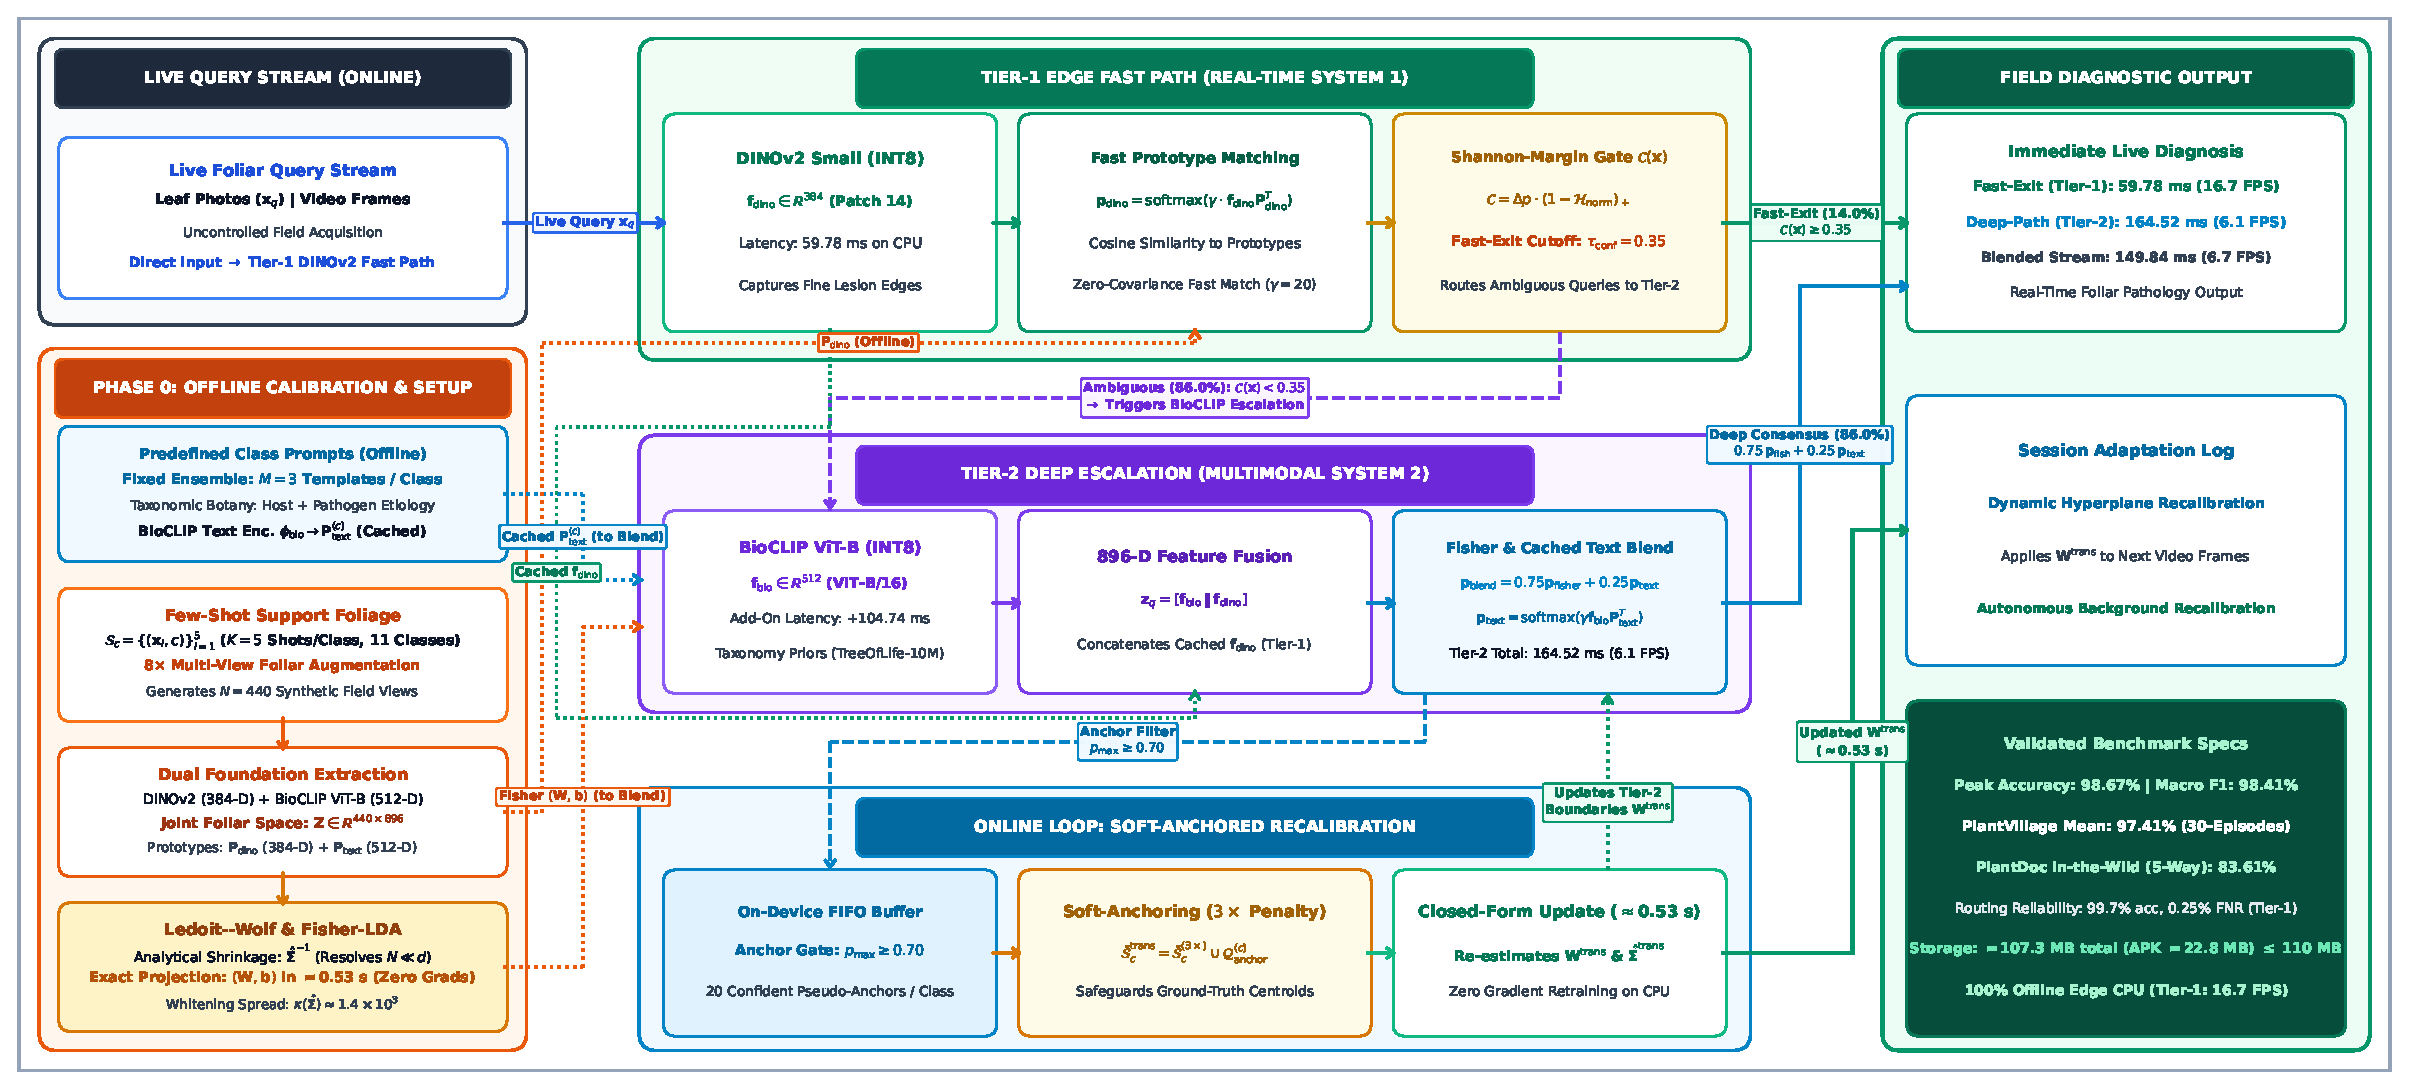
\includegraphics[width=0.95\textwidth]{fig_architecture.pdf}
\caption{Comprehensive architectural overview of BioDINO-Edge. Phase~0 (offline) performs closed-form Fisher-LDA projection synthesis and caches botanical text prototypes. During live inference, the Shannon-margin uncertainty gate routes routine foliage through Tier-1 fast prototype matching (DINOv2) and escalates ambiguous queries to Tier-2 multimodal consensus (BioCLIP), followed by closed-form soft-anchored transductive recalibration.}
\label{fig:architecture}
\end{figure*}

\subsection{Dual-Foundation Foliar Representation}
\label{sec:feature_extraction}
Effective diagnosis requires disentangling background foliar tissue from microscopic necrotic symptoms. Off-the-shelf vision encoders trained on general Web imagery lack taxonomic botanical concepts, while organism-level supervised models tend to prioritize whole-plant morphology over localized lesion pathology. We address this via dual-foundation extraction:

\subsubsection{Few-Shot Multi-View Support Augmentation}
To stabilize covariance estimation from only $K=5$ images per class, each support leaf $\mathbf{x} \in \mathcal{S}_c$ is resized to $224 \times 224$, normalized, and passed eight times through a stochastic augmentation pipeline approximating field variations. The pipeline applies random horizontal and vertical flips, random rotations within $\pm 15^\circ$, and color jitter (brightness, contrast, and saturation factors of 0.2). This generates 8 views per image, yielding $|\tilde{\mathcal{S}}_c| = 8K = 40$ augmented views per class, or $N = 40C = 440$ total support vectors ($N=440 \approx d/2 = 448$), which stabilizes covariance condition numbers. The eight views of a leaf are correlated pseudo-replicates of the same source image rather than independent observations; Section~\ref{sec:shrinkage} analyzes the consequences for shrinkage estimation, and Section~\ref{sec:aug_sensitivity} reports a sensitivity study over view count and augmentation type.

\subsubsection{Dual-Foundation Embedding Fusion}
Each augmented support view $\tilde{\mathbf{x}} \in \tilde{\mathcal{S}}_c$ is passed through frozen foundation backbones. DINOv2 Small ($14\times 14$ patches) \cite{oquab2023dinov2} and BioCLIP (the ViT-B/16 variant with $16\times16$-pixel patches, pretrained on TreeOfLife-10M) \cite{stevens2024bioclip} extract $\ell_2$-normalized spatial and organismal botanical vectors:
\begin{equation}
    \mathbf{f}_{\text{dino}} = \frac{\phi_{\text{dino}}(\tilde{\mathbf{x}})}{\|\phi_{\text{dino}}(\tilde{\mathbf{x}})\|_2} \in \mathbb{R}^{384}, \quad
    \mathbf{f}_{\text{bio}} = \frac{\phi_{\text{bio}}(\tilde{\mathbf{x}})}{\|\phi_{\text{bio}}(\tilde{\mathbf{x}})\|_2} \in \mathbb{R}^{512}
\end{equation}
Concatenating both normalized embeddings yields an 896-dimensional joint descriptor:
\begin{equation}
    \mathbf{z} = [\mathbf{f}_{\text{bio}} \,\|\, \mathbf{f}_{\text{dino}}] \in \mathbb{R}^{896}
\end{equation}
Visual prototypes for each encoder are computed via empirical support averaging:
\begin{equation}
    \mathbf{P}_{\text{enc}}^{(c)} = \text{Normalize}\left(\frac{1}{|\tilde{\mathcal{S}}_c|}\sum_{\tilde{\mathbf{x}} \in \tilde{\mathcal{S}}_c} \mathbf{f}_{\text{enc}}(\tilde{\mathbf{x}})\right), \quad \text{enc} \in \{\text{dino}, \text{bio}\}
\end{equation}
producing prototype matrices $\mathbf{P}_{\text{dino}} \in \mathbb{R}^{C \times 384}$ and $\mathbf{P}_{\text{bio,vis}} \in \mathbb{R}^{C \times 512}$.

\subsubsection{Botanical Taxonomic Prompts \& Syntactic Negation Neutralization}
BioCLIP provides a shared vision--language space. However, generating textual descriptions or running language decoders on edge devices at runtime would introduce unacceptable latency and memory consumption. We therefore predefine $M=3$ Latin botanical prompt ensembles $\{T_c^{(m)}\}_{m=1}^M$ offline for each disease category $c \in \{1, \dots, C\}$. Each template integrates three botanical dimensions:
\begin{enumerate}
    \item \textbf{Host Binomial Nomenclature:} Botanical genus and species (e.g., \textit{Malus domestica}, \textit{Vitis vinifera}, \textit{Solanum tuberosum}).
    \item \textbf{Causal Pathogen Etiology:} Pathogenic fungal, bacterial, or oomycete binomials (e.g., \textit{Venturia inaequalis}, \textit{Guignardia bidwellii}, \textit{Phytophthora infestans}).
    \item \textbf{Macroscopic Lesion Morphology:} Diagnostic foliar symptoms (e.g., ``olive-green velvety lesions'', ``tiger-stripe interveinal chlorosis'', ``target-board concentric rings'').
\end{enumerate}

Importantly, syntactic negations (e.g., ``healthy leaf without lesions'' or ``no necrotic spots'') are strictly excluded. Vision-language models exhibit documented compositional weaknesses regarding negation \cite{radford2021clip, yuksekgonul2023when, alhamoud2025vision}: high-density pathological tokens (e.g., \textit{lesion}, \textit{necrotic}) dominate embedding directions, pulling healthy leaf representations toward diseased clusters and inflating false-negative rates to 2.3\%. We neutralize this by using positive morphological descriptors of cellular vigor (e.g., ``flawless emerald lamina'', ``intact smooth venation'', ``clean vigorous green foliage''), reducing the clinical false-negative rate to 0.702\%.

During Phase~0 offline calibration, each prompt ensemble is encoded by BioCLIP's text encoder $\phi_{\text{bio,txt}}(\cdot)$, averaged, and $\ell_2$-normalized:
\begin{equation}
    \mathbf{P}_{\text{text}}^{(c)} = \text{Normalize}\left(\frac{1}{M}\sum_{m=1}^M \phi_{\text{bio,txt}}(T_c^{(m)})\right) \in \mathbb{R}^{512}
\end{equation}
The resulting matrix $\mathbf{P}_{\text{text}} \in \mathbb{R}^{C \times 512}$ is cached directly in the on-device model, requiring zero runtime text tokenization or language processing overhead.

\subsection{Closed-Form Analytical Adaptation via Regularized Fisher-LDA}
\label{sec:fisher_adaptation}

\subsubsection{Multiclass Fisher Linear Discriminant Formulation}
Standard metric few-shot approaches (e.g., Prototypical Networks \cite{snell2017prototypical} or Tip-Adapter \cite{zhang2022tip}) classify queries using Euclidean or cosine distances to class centroids $\boldsymbol{\mu}_c = \frac{1}{|\tilde{\mathcal{S}}_c|}\sum_{\mathbf{z} \in \tilde{\mathcal{S}}_c}\mathbf{z}$. This implicitly assumes uniform variance across all directions ($\mathbf{\Sigma} = \mathbf{I}$). In foliar pathology, however, within-class variance is strongly non-uniform across directions: a few dominant eigen-directions carry most of the shared vegetative variation, with a measured condition number $\kappa \approx 1.4\times10^{3}$ on the canonical support (Table~\ref{tab:aug_sensitivity}). Standard cosine similarity weights all directions equally and is therefore dominated by these high-variance background components, misclassifying distinct diseases of the same host species. The regularized Fisher-LDA projection (Section~\ref{sec:shrinkage}) resolves this by weighting features by the inverse covariance $\hat{\mathbf{\Sigma}}^{-1}$, mathematically down-weighting shared leaf background and amplifying low-variance, discriminative lesion symptoms.

Multiclass Fisher-LDA \cite{fisher1936use, rao1948utilization} finds an optimal projection matrix $\mathbf{W} \in \mathbb{R}^{C \times d}$ and bias vector $\mathbf{b} \in \mathbb{R}^C$ maximizing between-class scatter $\mathbf{S}_B$ relative to within-class scatter $\mathbf{S}_W$:
\begin{equation}
    \label{eq:fisher_weights}
    \mathbf{W} = [\boldsymbol{\mu}_1, \dots, \boldsymbol{\mu}_C]^T \hat{\mathbf{\Sigma}}^{-1}, \quad
    b_c = -\frac{1}{2} \boldsymbol{\mu}_c^T \hat{\mathbf{\Sigma}}^{-1} \boldsymbol{\mu}_c - \log C
\end{equation}
where $\hat{\mathbf{\Sigma}}$ denotes the pooled within-class covariance matrix and uniform class priors ($\pi_c = 1/C$) are assumed.

\subsubsection{The Small-Sample Singularity Problem ($N \ll d$)}
Evaluating \eqref{eq:fisher_weights} requires inverting the empirical pooled within-class scatter matrix across all $C=11$ classes:
\begin{equation}
    \mathbf{S}_W = \frac{1}{N - C}\sum_{c=1}^C \sum_{\mathbf{z} \in \tilde{\mathcal{S}}_c} (\mathbf{z} - \boldsymbol{\mu}_c)(\mathbf{z} - \boldsymbol{\mu}_c)^T \in \mathbb{R}^{d \times d}
\end{equation}
The denominator $N - C = 440 - 11 = 429$ represents degrees of freedom remaining after estimating $C$ class centroids from $N$ samples. In our setting, feature dimensionality $d=896$ exceeds available degrees of freedom ($429$). By fundamental linear algebra:
\begin{equation}
    \text{rank}(\mathbf{S}_W) \le \min(d, N - C) = 429 < 896
\end{equation}
Consequently, $\mathbf{S}_W$ has nullity of at least $896 - 429 = 467$, possessing at least 467 eigenvalues equal to zero ($\det(\mathbf{S}_W) = 0$). The matrix is strictly singular, rendering standard Fisher-LDA mathematically impossible to invert directly.

\subsubsection{Analytical Ledoit--Wolf Covariance Shrinkage}
\label{sec:shrinkage}
Rather than resorting to heuristic regularization (e.g., grid search over $\mathbf{S}_W + \epsilon \mathbf{I}$), we regularize $\mathbf{S}_W$ using analytical Ledoit--Wolf shrinkage \cite{ledoit2004well}, which contracts $\mathbf{S}_W$ toward a well-conditioned spherical target:
\begin{equation}
    \hat{\mathbf{\Sigma}} = (1 - \rho^*)\mathbf{S}_W + \rho^* \nu \mathbf{I}_{d}, \quad \nu = \frac{1}{d}\text{Tr}(\mathbf{S}_W)
    \label{eq:lw_target}
\end{equation}
The optimal shrinkage intensity $\rho^* \in (0, 1]$ is determined in closed form by minimizing expected quadratic Frobenius risk:
\begin{equation}
    \rho^* = \min\left(1, \frac{\sum_{i=1}^N \|(\mathbf{z}_i - \boldsymbol{\mu}_{c_i})(\mathbf{z}_i - \boldsymbol{\mu}_{c_i})^T - \mathbf{S}_W\|_F^2}{N^2 \left[\text{Tr}(\mathbf{S}_W^2) - \frac{1}{d}\text{Tr}^2(\mathbf{S}_W)\right]}\right)
    \label{eq:lw_shrinkage}
\end{equation}
Because all zero eigenvalues of $\mathbf{S}_W$ are shifted to strictly positive values $\tilde{\lambda}_i = (1 - \rho^*)\lambda_i + \rho^* \nu \ge \rho^* \nu > 0$, the regularized matrix $\hat{\mathbf{\Sigma}}$ is guaranteed to be strictly positive-definite and well-conditioned. Its inverse $\hat{\mathbf{\Sigma}}^{-1}$ is solved stably via Cholesky decomposition ($\hat{\mathbf{\Sigma}} = \mathbf{L}\mathbf{L}^T$). Evaluating a query vector $\mathbf{z}$ via $\mathbf{l}_{\text{fisher}} = \mathbf{z}\mathbf{W}^T + \mathbf{b}$ requires only $C \cdot d = 11 \times 896 = 9{,}856$ multiply-accumulate operations (one MAC = one multiply plus one add = 2 FLOPs, hence $\approx 19.7$\,kFLOPs), executing in $<$0.01\,ms on an edge CPU.

Weighting by $\hat{\mathbf{\Sigma}}^{-1}$ acts as a whitening transform: each eigen-direction of $\hat{\mathbf{\Sigma}}$ with variance $\lambda_i$ is rescaled by $1/\lambda_i$, so directions carrying the largest shared within-class variance receive the smallest weights and low-variance directions the largest. The spread of these weights is exactly the condition number
\begin{equation}
    \kappa(\hat{\mathbf{\Sigma}}) = \lambda_{\max}(\hat{\mathbf{\Sigma}}) / \lambda_{\min}(\hat{\mathbf{\Sigma}}),
    \label{eq:whitening_spread}
\end{equation}
measured as $1435.6 \pm 310.2$ over the 30 canonical episodes on the 8-view augmented support (Table~\ref{tab:aug_sensitivity}). Because the eigen-directions of $\hat{\mathbf{\Sigma}}$ carry no semantic annotation, we report this defined spectral spread rather than direction-specific background or lesion multipliers: the regularized inverse down-weights dominant shared-variance directions relative to low-variance ones when forming discriminant boundaries, entirely in closed form.

\paragraph{Statistical dependence of augmented views.}
The $N=440$ support vectors are not $440$ independent observations: the eight views generated from one leaf image are conditionally dependent given that image, so the effective sample size lies between $55$ (one independent draw per leaf) and $440$. Both the analytical intensity $\rho^*$ of Eq.~\eqref{eq:lw_shrinkage} and the nominal $N-C=429$ degrees of freedom assume i.i.d.\ sampling and are therefore optimistic under this dependence---replication inflates $N$ without adding independent information, and the estimated intensity shrinks accordingly even though the covariance estimate gains no new evidence. Two safeguards limit the practical impact. First, shrinkage keeps $\hat{\mathbf{\Sigma}}$ strictly positive definite regardless of the nominal rank, so the closed-form solve remains well-posed at any effective sample size. Second, the transductive re-weighting of Section~\ref{sec:transductive} triples the canonical support relative to pseudo-labeled anchors, anchoring the fit to genuine observations. Section~\ref{sec:aug_sensitivity} quantifies the residual effect with a view-count and augmentation-type sensitivity study, including a pure-replication control that isolates the effect of dependence on the estimated intensity.

\subsection{Adaptive Two-Tier Classification and Edge Deployment}
\label{sec:edge_cascade}

\subsubsection{Tier-1 Fast Path and Shannon Uncertainty Gating}
For an incoming leaf image $\mathbf{x}$, Tier~1 extracts the normalized DINOv2 embedding $\mathbf{f}_{\text{dino}} \in \mathbb{R}^{384}$. Fast prototype logits are evaluated via temperature-scaled cosine similarity against visual prototypes $\mathbf{P}_{\text{dino}} \in \mathbb{R}^{C \times 384}$:
\begin{equation}
    \label{eq:tier1_logits}
    \mathbf{l}_{\text{dino}} = \gamma \cdot \left(\mathbf{f}_{\text{dino}} \mathbf{P}_{\text{dino}}^T\right), \quad \gamma = 20.0
\end{equation}
Applying softmax yields fast posterior probabilities:
\begin{equation}
    \label{eq:tier1_softmax}
    \mathbf{p}_{\text{dino}} = \text{softmax}(\mathbf{l}_{\text{dino}}) \in \Delta^{C-1}
\end{equation}
To strictly minimize edge computational overhead on routine foliage, Tier~1 deliberately employs zero-covariance cosine prototype matching rather than discriminant projection, reserving regularized Fisher-LDA exclusively for Tier-2 escalation where ambiguous queries require full covariance debiasing. The initial Tier-1 prediction is $\hat{y}_{\text{tier1}} = \arg\max_c p_{\text{dino}, c}$.

To evaluate prediction certainty without additional forward passes, we formulate a joint margin-entropy confidence score $\mathcal{C}(\mathbf{x}) \in [0, 1]$:
\begin{equation}
    \label{eq:shannon_gate}
    \mathcal{C}(\mathbf{x}) = \left(p_{\text{dino}, (1)} - p_{\text{dino}, (2)}\right) \cdot \left(1.0 - \mathcal{H}_{\text{norm}}(\mathbf{x})\right)_+
\end{equation}
where $p_{\text{dino}, (1)}$ and $p_{\text{dino}, (2)}$ denote top-1 and top-2 posteriors, $(\cdot)_+ = \max(0, \cdot)$, and $\mathcal{H}_{\text{norm}}(\mathbf{x})$ is normalized Shannon entropy \cite{shannon1948mathematical}:
\begin{equation}
    \mathcal{H}_{\text{norm}}(\mathbf{x}) = -\frac{1}{\log C} \sum_{c=1}^C p_{\text{dino}, c} \log(p_{\text{dino}, c} + \epsilon)
\end{equation}
with numerical stability constant $\epsilon = 10^{-12}$. Because Shannon entropy is bounded by $\log C$, $\mathcal{H}_{\text{norm}} \in [0,1]$ and $1-\mathcal{H}_{\text{norm}}$ is non-negative in exact arithmetic (the $\epsilon$-regularized logarithm can only underestimate the entropy); the $(\cdot)_+$ operator in Eq.~\eqref{eq:shannon_gate} is thus a floating-point safeguard against round-off, not a theoretical correction. When a leaf query is ambiguous (near-uniform distribution), $\mathcal{H}_{\text{norm}} \to 1.0$ and margin $\to 0$, driving $\mathcal{C}(\mathbf{x}) \to 0$. If $\mathcal{C}(\mathbf{x}) \ge \tau_{\text{conf}}$ (with threshold $\tau_{\text{conf}} = 0.35$ selected on held-out development episodes; Section~\ref{sec:calibration}), Tier-1 exits immediately at 59.78\,ms ($\approx$16.7\,FPS). Approximately 14.0\% of PlantVillage queries---the highest-confidence subset---exit through this fast path; the remainder escalate to Tier-2.

\subsubsection{Tier-2 Multimodal Consensus Escalation}
When $\mathcal{C}(\mathbf{x}) < \tau_{\text{conf}}$, the query escalates to Tier-2. BioCLIP ViT-B extracts $\mathbf{f}_{\text{bio}} \in \mathbb{R}^{512}$, forming $\mathbf{z} = [\mathbf{f}_{\text{bio}} \,\|\, \mathbf{f}_{\text{dino}}] \in \mathbb{R}^{896}$. Discriminant visual posteriors $\mathbf{p}_{\text{fisher}} = \text{softmax}(\mathbf{z}\mathbf{W}^T + \mathbf{b})$ and taxonomic text posteriors $\mathbf{p}_{\text{text}} = \text{softmax}(\gamma \cdot \mathbf{f}_{\text{bio}}\mathbf{P}_{\text{text}}^T)$ are fused at a 0.75 / 0.25 consensus ratio:
\begin{equation}
    \label{eq:multimodal_blend}
    \mathbf{p}_{\text{blend}} = 0.75 \, \mathbf{p}_{\text{fisher}} + 0.25 \, \mathbf{p}_{\text{text}}
\end{equation}
yielding the final consensus diagnosis $\hat{y} = \arg\max_c p_{\text{blend}, c}$.

\subsubsection{Soft-Anchored Transductive Recalibration}
\label{sec:transductive}
In 5-shot calibration, centroids $\boldsymbol{\mu}_c$ are estimated from five support leaves. Diurnal illumination changes, shadows, and symptom progression introduce prototype shift between initial support images and field queries. To adapt without manual labels, confident Tier-2 queries satisfying $\max_c p_{\text{blend}, c} \ge 0.70$ are buffered into an on-device FIFO queue as reference anchors $\mathcal{Q}_{\text{anchor}}^{(c)}$, capped at 20 anchors per class. Ground-truth support samples receive a $3\times$ weight factor to prevent pseudo-label drift:
\begin{equation}
    \tilde{\mathcal{S}}_c^{\text{trans}} = \tilde{\mathcal{S}}_c^{(3\times)} \cup \mathcal{Q}_{\text{anchor}}^{(c)}
\end{equation}
When the buffer reaches capacity during scouting, updated centroids $\boldsymbol{\mu}_c^{\text{trans}}$ and pooled scatter matrix $\mathbf{S}_W^{\text{trans}}$ are re-estimated. Analytical shrinkage parameter $\rho^*$ is recomputed, and updated projection parameters $(\mathbf{W}^{\text{trans}}, \mathbf{b}^{\text{trans}})$ are resolved via Cholesky substitution in $\approx$0.53\,s in the background (measured on-device, Table~\ref{tab:adaptation_breakdown}), updating subsequent Tier-2 decisions while Tier-1 continues operating with static prototypes. The three constants are set from a one-factor-at-a-time sweep over the 30 evaluation episodes (Section~\ref{sec:transductive_validation}, Table~\ref{tab:transductive_sensitivity}): in-domain accuracy spans 97.21--97.44\% for support weights $1\times$--$10\times$, $\tau = 0.70$ lies on a plateau bounded by anchor-coverage collapse, and 20 anchors per class sit at the knee of the capacity curve; anchor purity at the deployed threshold is 98.15\%.

\subsection{Algorithmic Pipeline and Complexity Analysis}
\label{sec:complexity}
The complete end-to-end execution flow is formalized in Algorithm~\ref{alg:biodino}. We analyze computational complexity across both operational phases:
\begin{itemize}
    \item \textbf{Offline Calibration Complexity:} Feature extraction across $N=440$ views requires $O(N \cdot (C_{\text{dino}} + C_{\text{bio}}))$ FLOPs and dominates the wall-clock cost ($\approx$88\,s on-device, reported separately). Scatter matrix computation requires $O(N d^2)$ operations. The Ledoit--Wolf shrinkage intensity is evaluated in closed form via the Frobenius identity $\sum_i \|\mathbf{x}_i \mathbf{x}_i^T - \mathbf{S}\|_F^2 = \sum_i \|\mathbf{x}_i\|^4 - N \|\mathbf{S}\|_F^2$, reducing it to $O(N d)$. Inverting the positive-definite matrix via Cholesky decomposition requires $O(d^3 / 3)$ operations. For $d=896$, $d^3 / 3 \approx 2.4 \times 10^8$ operations; on the physical edge CPU (pure-Java EJML) the Cholesky factorization alone measures $\approx$332\,ms and the full algebraic recalibration (covariance, shrinkage, Cholesky, solve) $\approx$0.53\,s, gradient-free and sub-second (Table~\ref{tab:adaptation_breakdown}).
    \item \textbf{Online Inference Complexity:} Tier-1 forward pass requires $C_{\text{dino}}$ ($\approx 4.6$\,GFLOPs), yielding a measured fast-exit latency of $T_1 = 59.78$\,ms ($\approx$16.7\,FPS) on the physical Android testbed (Section~\ref{sec:edge_hardware}). Dot-product prototype matching requires $C \cdot d_{\text{dino}} = 11 \times 384 \approx 4.2$\,kFLOPs ($<$0.002\,ms), and entropy gating requires $O(C)$ operations ($<$0.001\,ms). Upon escalation, BioCLIP adds a measured incremental encoder cost of $\Delta T_{\text{bio}} = 104.74$\,ms ($C_{\text{bio}} \approx 17.6$\,GFLOPs), since the Tier-1 DINOv2 embedding is cached and reused rather than recomputed. The joint Fisher-LDA projection is fused into the same Tier-2 ONNX graph ($C \cdot d = 11 \times 896 \approx 9.8$\,kFLOPs, negligible). The complete end-to-end Tier-2 path for an escalated query therefore costs $T_2 = T_1 + \Delta T_{\text{bio}} = 164.52$\,ms ($\approx$6.1\,FPS). With 14.0\% of queries exiting at Tier-1 (Section~\ref{sec:calibration}), the routing-weighted average latency across field streams is:
    \begin{align}
        \bar{T} &= 0.140 \cdot T_1 + 0.860 \cdot T_2 \nonumber \\
        &= 0.140 \cdot 59.78\,\text{ms} + 0.860 \cdot 164.52\,\text{ms} \nonumber \\
        &\approx 149.84\,\text{ms}
    \end{align}
    delivering $\approx$6.7 frames per second at the system level; the $\approx$16.7\,FPS figure applies only to the Tier-1 fast-exit path. These are interactive handheld-scouting rates (one diagnosis per captured frame), not continuous real-time video; sustained throughput under thermal load is reported in Section~\ref{sec:edge_hardware}.
\end{itemize}

\begin{figure*}[htbp]
\centering
\fbox{
\begin{minipage}{0.95\textwidth}
\small
\textbf{Algorithm 1: BioDINO-Edge Offline Calibration and Online Adaptive Cascaded Inference}
\vspace{4pt}
\hrule
\vspace{4pt}
\textbf{Input:} Support set $\mathcal{S} = \{(\mathbf{x}_i, y_i)\}_{i=1}^{CK}$ ($K=5$); unannotated query stream $\{\mathbf{x}_q\}$; prompt bank $\{T_c^{(m)}\}$; threshold $\tau_{\text{conf}}=0.35$. \\
\textbf{Output:} Predicted disease class $\hat{y}_q \in \{1, \dots, C\}$ and confidence score $\mathcal{C}(\mathbf{x}_q)$ for each query.

\vspace{2pt}
\textbf{// Phase 0: Offline Analytical Support Calibration (Zero Backpropagation)}
\begin{enumerate}
    \setlength{\itemsep}{1pt}
    \item Expand each support leaf $\mathbf{x} \in \mathcal{S}_c$ into 8 stochastic views $\tilde{\mathcal{S}}_c$ via affine flips, rotations ($\pm 15^\circ$), and color jitter ($N=440$).
    \item Extract normalized vectors $\mathbf{f}_{\text{dino}} \in \mathbb{R}^{384}$ and $\mathbf{f}_{\text{bio}} \in \mathbb{R}^{512}$; concatenate to $\mathbf{z} = [\mathbf{f}_{\text{bio}} \,\|\, \mathbf{f}_{\text{dino}}] \in \mathbb{R}^{896}$.
    \item Compute DINO prototypes $\mathbf{P}_{\text{dino}} \in \mathbb{R}^{C \times 384}$ and encode cached text prototypes $\mathbf{P}_{\text{text}} \in \mathbb{R}^{C \times 512}$ using \eqref{eq:tier1_logits}--\eqref{eq:shannon_gate}.
    \item Compute empirical class centroids $\boldsymbol{\mu}_c$ and pooled within-class scatter matrix $\mathbf{S}_W \in \mathbb{R}^{896 \times 896}$.
    \item Calculate Ledoit--Wolf analytical shrinkage intensity $\rho^*$ and form $\hat{\mathbf{\Sigma}} = (1 - \rho^*)\mathbf{S}_W + \rho^* \nu \mathbf{I}_{896}$.
    \item Invert $\hat{\mathbf{\Sigma}}$ via Cholesky decomposition and evaluate projection parameters $\mathbf{W} = [\boldsymbol{\mu}_1, \dots, \boldsymbol{\mu}_C]^T \hat{\mathbf{\Sigma}}^{-1}$ and $\mathbf{b}$.
\end{enumerate}

\vspace{2pt}
\textbf{// Phase 1: Online Adaptive Cascaded Inference}
\begin{enumerate}
    \setcounter{enumi}{6}
    \setlength{\itemsep}{1pt}
    \item For incoming query $\mathbf{x}_q$, extract normalized DINOv2 embedding $\mathbf{f}_{\text{dino}} \in \mathbb{R}^{384}$ (59.78\,ms).
    \item Evaluate fast prototype logits $\mathbf{l}_{\text{dino}} = \gamma (\mathbf{f}_{\text{dino}}\mathbf{P}_{\text{dino}}^T)$ and posteriors $\mathbf{p}_{\text{dino}} = \text{softmax}(\mathbf{l}_{\text{dino}})$.
    \item Compute confidence score $\mathcal{C}(\mathbf{x}_q) = (p_{(1)} - p_{(2)}) \cdot (1.0 - \mathcal{H}_{\text{norm}}(\mathbf{x}_q))_+$.
    \item \textbf{if} $\mathcal{C}(\mathbf{x}_q) \ge \tau_{\text{conf}}$ (0.35) \textbf{then}
    \item \quad Return $\hat{y}_q = \arg\max_c p_{\text{dino}, c}$ \textbf{(Tier-1 Fast-Exit, 59.78\,ms, $\approx$16.7\,FPS)}.
    \item \textbf{else} // Escalate to Tier-2 Deep Multimodal Analysis
    \item \quad Extract BioCLIP visual embedding $\mathbf{f}_{\text{bio}} \in \mathbb{R}^{512}$; concatenate $\mathbf{z}_q = [\mathbf{f}_{\text{bio}} \,\|\, \mathbf{f}_{\text{dino}}] \in \mathbb{R}^{896}$.
    \item \quad Compute visual posterior $\mathbf{p}_{\text{fisher}} = \text{softmax}(\mathbf{z}_q \mathbf{W}^T + \mathbf{b})$ and text posterior $\mathbf{p}_{\text{text}} = \text{softmax}(\gamma \mathbf{f}_{\text{bio}}\mathbf{P}_{\text{text}}^T)$.
    \item \quad Form consensus posterior $\mathbf{p}_{\text{blend}} = 0.75 \, \mathbf{p}_{\text{fisher}} + 0.25 \, \mathbf{p}_{\text{text}}$; return $\hat{y}_q = \arg\max_c p_{\text{blend}, c}$.
    \item \quad \textbf{if} $\max_c p_{\text{blend}, c} \ge 0.70$ \textbf{then} buffer $\mathbf{z}_q$ into class anchor queue $\mathcal{Q}_{\text{anchor}}^{(\hat{y}_q)}$.
    \item \quad \textbf{if} anchor buffer reaches update capacity \textbf{then} execute transductive update in background.
    \item \textbf{end if}
\end{enumerate}
\vspace{2pt}
\end{minipage}
}
\refstepcounter{algocounter}\label{alg:biodino}
\end{figure*}

\subsection{Two-Tier Quantized Edge Model Packaging and Android Architecture}
\label{sec:packaging}
Agricultural scouting hardware operates under rigorous physical constraints: onboard Flash memory is shared with flight telemetry and sensor buffers, while remote rural fields lack Internet connectivity for cloud offloading. BioDINO-Edge is partitioned into two 8-bit integer (INT8) quantized Open Neural Network Exchange (ONNX) binaries (all footprint values are in MiB, i.e., $1\,\text{MB}=2^{20}$ bytes):
\begin{itemize}
    \item \textbf{Tier 1 Standalone Engine} (\path{biodino_mobile_int8.onnx}): A $\approx$22.0\,MB on-disk binary ($\approx$15.1\,MB compressed inside the APK) packaging DINOv2 Small INT8, calibrated Phase~0 prototypes, and the Shannon confidence gate with the ONNX Runtime C++ execution provider. Bundled directly into a standalone $\approx$22.8\,MB Android application package (APK), it enables immediate offline foliar diagnosis. Runtime RAM is dominated by the ONNX Runtime arena rather than the binary size and is measured separately (peak process PSS $\approx$497\,MB, Section~\ref{sec:edge_hardware}).
    \item \textbf{Tier 2 Companion Module} (\path{biodino_companion_int8.onnx}): An $\approx$85.3\,MB companion model packaging BioCLIP ViT-B INT8 and the 896-D Fisher projection matrix, installed on-demand when high-precision multimodal escalation is required. The total combined on-disk model footprint is $\approx$107.3\,MB, below the 110\,MB Internet-of-Things (IoT) \emph{storage} budget; this is a flash/OTA size constraint, not a runtime RAM bound (runtime memory is reported in Section~\ref{sec:edge_hardware}).
\end{itemize}

% =============================================================================
% 3. EXPERIMENTAL SETUP
% =============================================================================
\section{Experimental Setup}
\label{sec:experiments_setup}

\subsection{Datasets and Diagnostic Pathology Coverage}
\label{sec:datasets}
We evaluate BioDINO-Edge across two distinct foliar pathology regimes:

\subsubsection{PlantVillage Controlled Benchmark (Laboratory Regime)}
From the standard PlantVillage repository \cite{hughes2012plantvillage}, we construct a curated 11-class diagnostic subset comprising 9,385 foliar images across three economically critical crops: Apple (\textit{Malus domestica}), Grape (\textit{Vitis vinifera}), and Potato (\textit{Solanum tuberosum}). The 11 classes span healthy foliage and 8 fungal/bacterial/oomycete pathologies: Apple Scab (\textit{Venturia inaequalis}), Apple Black Rot (\textit{Botryosphaeria obtusa}), Apple Cedar Rust (\textit{Gymnosporangium juniperi-virginianae}), Apple Healthy, Grape Black Rot (\textit{Guignardia bidwellii}), Grape Esca / Black Measles (\textit{Phaeomoniella chlamydospora}), Grape Leaf Blight (\textit{Pseudocercospora vitis}), Grape Healthy, Potato Early Blight (\textit{Alternaria solani}), Potato Late Blight (\textit{Phytophthora infestans}), and Potato Healthy. For few-shot calibration, 5 support leaves per class ($K=5$) are randomly sampled (55 total), strictly isolating the remaining 9,330 images as unseen query test leaves. Neither support nor test splits were involved in pretraining the frozen foundation backbones.

\subsubsection{PlantDoc In-The-Wild Benchmark (Field Regime)}
To evaluate field-domain robustness under complex agricultural noise (e.g., specular solar glare, canopy shading, soil clutter, overlapping foliage, and motion blur), we evaluate on the in-the-wild PlantDoc benchmark \cite{singh2020plantdoc}. PlantDoc comprises 2,588 foliar images spanning 27 pathology classes across 13 botanical species, partitioned officially into:
\begin{itemize}
    \item \textbf{Official Training Repository ($\mathcal{D}_{\text{train}}^{\text{PlantDoc}}$):} 2,336 in-the-wild images across all 27 target classes, used only as the source of few-shot support samples.
    \item \textbf{Official Test Benchmark ($\mathcal{D}_{\text{test}}^{\text{PlantDoc}}$):} 252 unconstrained field images across the 27 classes, captured with handheld mobile devices under ambient field illumination in Indian agricultural orchards.
\end{itemize}
Support sets are drawn only from $\mathcal{D}_{\text{train}}^{\text{PlantDoc}}$ and query sets only from $\mathcal{D}_{\text{test}}^{\text{PlantDoc}}$, so the two never overlap ($\mathcal{S} \cap \mathcal{Q} = \emptyset$). We evaluate under two few-shot regimes:
\begin{enumerate}
    \item \textbf{5-Way 5-Shot Episodic Benchmark:} Following standard few-shot evaluation protocols \cite{snell2017prototypical,zhou2026vsf}, we conduct 50 independent Monte Carlo episodes. In each episode $e$, 5 classes are sampled uniformly at random without replacement ($\mathcal{C}_e \subset \{1, \dots, 27\}$). The support set $\mathcal{S}_e$ consists of 5 labeled leaves per class ($5 \times 5 = 25$ total) randomly sampled from the respective class directories in $\mathcal{D}_{\text{train}}^{\text{PlantDoc}}$. The query set $\mathcal{Q}_e$ comprises all test images in $\mathcal{D}_{\text{test}}^{\text{PlantDoc}}$ corresponding to those 5 sampled classes (averaging 46.7 query leaves per episode), ensuring $\mathcal{S}_e \cap \mathcal{Q}_e = \emptyset$.
    \item \textbf{27-Way All-Class Simultaneous Stress Test:} All 27 classes are evaluated simultaneously (random chance: $1/27 \approx 3.70\%$). The model receives 5 support leaves per category ($5 \times 27 = 135$ total) sampled strictly from $\mathcal{D}_{\text{train}}^{\text{PlantDoc}}$ (expanded via 8-view multi-scale cropping and color jitter to $N = 1{,}080$ feature vectors) and evaluates on all 252 unconstrained field queries from $\mathcal{D}_{\text{test}}^{\text{PlantDoc}}$ in closed form without gradient backpropagation ($\mathcal{S} \cap \mathcal{Q} = \emptyset$).
\end{enumerate}

\subsection{Data Integrity, Hyperparameter Provenance, and Leakage Safeguards}
\label{sec:integrity}
We enforce five safeguards against data leakage and circular tuning:
\begin{itemize}
    \item \textbf{Adaptation Settings Defined:} We distinguish three settings: (i) \emph{few-shot adaptation with labeled target-domain support}, in which the $K$ support leaves per class come from the same domain as the queries (all PlantVillage regimes, and the PlantDoc benchmark whose support is drawn from the PlantDoc training split); (ii) \emph{cross-domain few-shot adaptation}, in which support comes from a source domain and queries from a different target domain (PlantVillage$\rightarrow$PlantDoc in Zhao \textit{et al.}, Table~\ref{tab:literature}), which we do not run; and (iii) \emph{transductive recalibration}, which adds no labels and uses only pseudo-labeled streaming queries (Section~\ref{sec:transductive}). The only cross-domain element of our PlantDoc protocol is the transfer of hyperparameters selected on PlantVillage; the support itself is target-domain.
    \item \textbf{Disjoint Support-Query Separation:} Support and query sets are disjoint ($\mathcal{S} \cap \mathcal{Q} = \emptyset$) in both regimes: PlantVillage isolates 55 support leaves from the 9,330 test images, and PlantDoc draws all 135 support samples from $\mathcal{D}_{\text{train}}^{\text{PlantDoc}}$ and all 252 queries from $\mathcal{D}_{\text{test}}^{\text{PlantDoc}}$.
    \item \textbf{Zero-Tuning Analytical Regularization:} The Ledoit--Wolf shrinkage intensity $\rho^*$ follows in closed form from the support covariance (Eq.~\ref{eq:lw_shrinkage}); no hyperparameter search, cross-validation, or query/test tuning is involved.
    \item \textbf{Frozen Cross-Domain Hyperparameters:} The logit scale $\gamma = 20.0$, the Fisher-LDA blend weight $w_{\text{lda}} = 0.75$, and the routing threshold $\tau = 0.35$ were selected on held-out PlantVillage development episodes (0--14 tune, 15--29 test; Section~\ref{sec:calibration}) and frozen for all PlantDoc experiments, which use no validation split or tuning.
    \item \textbf{Unsupervised Transductive Anchoring:} The transductive module (Section~\ref{sec:transductive}) uses only streaming query features and predicted pseudo-labels. Query ground truth is withheld until after inference, when it is used solely to compute metrics.
    \item \textbf{Dual Inductive vs. Transductive Reporting:} Table~\ref{tab:comparative} reports both inductive performance (queries processed independently, without anchor updates) and transductive performance under identical splits. On the field-domain PlantDoc benchmark the inductive mode alone reaches 81.79\% $\pm$ 11.16\% (5-way 5-shot) and 55.16\% (27-way), so the reported performance does not depend on transductive anchor updates.
\end{itemize}

\subsection{Evaluation Protocols and Epidemiological Safety Metrics}
\label{sec:metrics}
Experiments on PlantVillage are evaluated over 30 independent Monte Carlo episodes with randomized support splits, reporting mean accuracy $\bar{x}$, standard deviation $\sigma$, 95\% confidence intervals ($95\%\,\text{CI} = \bar{x} \pm 1.96 \cdot \sigma / \sqrt{30}$), and peak single-episode accuracy. Because misclassification costs in precision agriculture are highly asymmetric, we evaluate epidemiological safety metrics alongside standard accuracy:
\begin{itemize}
    \item \textbf{Top-1 Accuracy \& Macro F1-Score:} The F1-score is the harmonic mean of precision and recall, macro-averaged across all classes to prevent frequent classes (e.g., Potato Early Blight with 995 queries) from masking errors on small or healthy classes (e.g., Potato Healthy with 147 queries).
    \item \textbf{False-Negative Disease Escape Rate (FNR):} The critical proportion of diseased leaves erroneously diagnosed as healthy: $\text{FNR} = \text{FN} / (\text{TP} + \text{FN})$, where FN and TP denote false-negative and true-positive counts, respectively. Undetected disease spread leads to catastrophic orchard devastation.
    \item \textbf{Cross-Species Confusion Rate:} The proportion of queries misattributed to an entirely different botanical family (e.g., classifying a potato leaf as an apple disease), indicating severe semantic collapse.
\end{itemize}

\subsection{Edge Hardware Testbed}
Hardware profiling runs on a physical Samsung Galaxy S24~FE (SM-S721B, Exynos~2400e / s5e9945, 10-core ARM64, 7.2\,GB RAM) under Android~17 (API~37). Runtime latency and memory benchmarks use ONNX Runtime~1.18.0 with per-channel INT8 quantization on the CPU, constrained to 4 intra-op / 2 inter-op threads with the NNAPI and GPU delegates disabled; the closed-form algebra runs in pure Java (EJML~0.43.1). Latency is timed with \texttt{SystemClock.elapsedRealtimeNanos} over 100 iterations after 10 warm-up passes, memory is the process PSS, and a 600\,s sustained soak plus a 60\,s cool-down before the algebra isolate thermal effects. Full configuration and measured results are reported in Section~\ref{sec:edge_hardware} (Tables~\ref{tab:device_spec}--\ref{tab:adaptation_breakdown}).

% =============================================================================
% 4. RESULTS AND DISCUSSION
% =============================================================================
\section{Results and Comparative Analysis}
\label{sec:results}

\subsection{Comparative Baseline Performance}
\label{sec:comparative_results}
To ensure a fair and reproducible comparison, we separate \emph{controlled re-runs} from \emph{literature-reported} values. Table~\ref{tab:comparative} re-runs every baseline ourselves on the \emph{identical} frozen BioCLIP+DINOv2 embeddings, support/query splits, random seeds, $K$-shot counts, and evaluation protocol as BioDINO-Edge; because no backbone is retrained, the comparison isolates the adaptation algorithm rather than the encoder. We evaluate two regimes on the PlantVillage 11-class novel subset (9{,}385 images): (i)~11-class simultaneous classification (30 Monte-Carlo episodes, seed $42+17e$, 5-shot support, all remaining images as queries), and (ii)~the standard 5-way $K$-shot episodic ladder ($K=1,5,10,15$; 50 episodes each, seed 42), which matches the measurement protocols of VSF~\cite{zhou2026vsf} (5-way 1/5-shot) and AgriFewNet~\cite{babu2025agrifewnet} (1/5/10/15-shot) so that our results can be compared \emph{in-regime}. The baselines are training-free and correctly referenced: Zero-Shot CLIP/BioCLIP~\cite{radford2021clip,stevens2024bioclip}, Tip-Adapter~\cite{zhang2022tip} ($\alpha{=}1.0,\beta{=}5.5$), Prototypical Networks~\cite{snell2017prototypical}, and SimpleShot~\cite{wang2019simpleshot}. Table~\ref{tab:literature} separately lists specialized architectures \emph{as reported} in their original publications; these use different encoders, class subsets, and splits, so they provide context only and are \emph{not} a controlled head-to-head. Full splits, seeds, model versions, and hyperparameters are given in \ref{app:repro}.

\begin{table*}[htbp]
\centering
\caption{Controlled few-shot comparison on the PlantVillage 11-class novel subset. \textbf{All methods use identical frozen BioCLIP+DINOv2 features, identical support/query splits, seeds, and protocol}; no backbone is retrained. 11-class: 30 episodes (seed $42{+}17e$, 5-shot); 5-way $K$-shot: 50 episodes per $K$ (seed 42). Acc.\ is mean $\pm$ std over episodes (\%); F1 is macro-mean (\%). Baselines are re-implemented and re-run by us; BioDINO-Edge 11-class values are the canonical reference run (Section~\ref{sec:transductive_validation}), reproduced by the provided script within 0.04\,pp (\ref{app:repro}). Prototypical Networks and SimpleShot coincide because Euclidean and cosine rankings are identical on $\ell_2$-normalized features. Bold: best mean.}
\label{tab:comparative}
\footnotesize
\begin{tabularx}{\textwidth}{l *{6}{>{\centering\arraybackslash}X}}
\toprule
& \multicolumn{2}{c}{\textbf{11-Class (30 ep.)}} & \multicolumn{4}{c}{\textbf{5-Way $K$-Shot (50 ep.\ each)}} \\
\cmidrule(lr){2-3} \cmidrule(lr){4-7}
\textbf{Method} & \textbf{Acc.} & \textbf{Macro F1} & \textbf{$K{=}1$} & \textbf{$K{=}5$} & \textbf{$K{=}10$} & \textbf{$K{=}15$} \\
\midrule
Zero-Shot CLIP/BioCLIP \cite{radford2021clip,stevens2024bioclip} & 19.18 $\pm$ 0.02 & 18.49 & 38.89 $\pm$ 12.78 & 38.86 $\pm$ 12.79 & 38.83 $\pm$ 12.81 & 38.79 $\pm$ 12.83 \\
Tip-Adapter \cite{zhang2022tip} & 49.97 $\pm$ 1.62 & 46.54 & 45.15 $\pm$ 13.42 & 68.63 $\pm$ 12.80 & 86.01 $\pm$ 7.49 & 93.23 $\pm$ 4.00 \\
Prototypical Networks \cite{snell2017prototypical} & 93.28 $\pm$ 1.24 & 92.47 & 88.44 $\pm$ 9.13 & 97.45 $\pm$ 2.03 & 98.35 $\pm$ 1.45 & 98.57 $\pm$ 1.27 \\
SimpleShot \cite{wang2019simpleshot} & 93.28 $\pm$ 1.24 & 92.47 & 88.44 $\pm$ 9.13 & 97.45 $\pm$ 2.03 & 98.35 $\pm$ 1.45 & 98.57 $\pm$ 1.27 \\
\midrule
BioDINO-Edge (Inductive) & 95.08 $\pm$ 1.27 & 94.51 & 88.45 $\pm$ 9.12 & 97.96 $\pm$ 1.85 & 99.10 $\pm$ 0.87 & 99.41 $\pm$ 0.60 \\
\textbf{BioDINO-Edge (Transductive, Ours)} & \textbf{97.41 $\pm$ 0.71} & \textbf{97.09} & \textbf{93.42 $\pm$ 6.83} & \textbf{98.77 $\pm$ 1.68} & \textbf{99.41 $\pm$ 0.60} & \textbf{99.63 $\pm$ 0.39} \\
\bottomrule
\end{tabularx}
\end{table*}

\begin{table*}[htbp]
\centering
\caption{Specialized agricultural few-shot architectures, \emph{as reported} in the original publications (not re-run by us). Encoders, class subsets, support/query splits, and preprocessing differ from our controlled protocol (Table~\ref{tab:comparative}); these values provide in-regime context only and do \emph{not} constitute a controlled head-to-head, so no direct superiority claim is drawn from them. AgriFewNet reports $K$-shot accuracy on PlantVillage/New PlantVillage; VSF reports 5-way $K$-shot; Zhao \textit{et al.} report cross-domain (PlantVillage$\rightarrow$PlantDoc) $K$-shot under a unified protocol.}
\label{tab:literature}
\small
\begin{tabularx}{\textwidth}{l l l X}
\toprule
\textbf{Method} & \textbf{Dataset} & \textbf{Regime} & \textbf{Reported Acc. (\%)} \\
\midrule
AgriFewNet \cite{babu2025agrifewnet} & PlantVillage / New PV & 1/5/10/15-shot & 87.3 / 94.8 / 97.1 / 98.2 \\
VSF \cite{zhou2026vsf} & PlantVillage & 5-way 1/5-shot & 79.01 / 90.51 \\
VSF \cite{zhou2026vsf} & PlantDoc & 5-way 1/5-shot & 59.82 / 70.61 \\
Zhao \textit{et al.} \cite{zhao2026lightweight} & PV $\rightarrow$ PlantDoc & 1/5-shot & 42.69 $\pm$ 0.62 / 54.24 $\pm$ 0.72 \\
\bottomrule
\end{tabularx}
\end{table*}

In the controlled 11-class regime (Table~\ref{tab:comparative}), Zero-Shot CLIP/BioCLIP reaches only 19.18\% because general pretraining cannot separate fine-grained lesions from healthy leaf mesophyll, and the training-free Tip-Adapter cache reaches 49.97\%. Centroid-based Prototypical Networks and SimpleShot are already strong (93.28\%), confirming that the frozen BioCLIP+DINOv2 features are highly discriminative; BioDINO-Edge improves on them through regularized Fisher-LDA (95.08\% inductive) and closed-form transductive recalibration (97.41\%), a 2.33-point paired gain over the inductive mode on identical episodes (Section~\ref{sec:transductive_validation}). Gradient-based fine-tuning such as CLIP+LoRA \cite{hu2022lora} would require GPU backpropagation and optimizer states, which our gradient-free closed-form adaptation avoids entirely. In the easier 5-way regime the centroid baselines already reach 97.45\% (5-shot) and 98.57\% (15-shot), so the margin narrows; BioDINO-Edge remains best at every $K$ (98.77\% at 5-shot, 99.63\% at 15-shot), and its transductive gain is largest in the hardest 1-shot setting (93.42\% vs.\ 88.44\% for Prototypical Networks).

For context, Table~\ref{tab:literature} lists specialized architectures \emph{as reported} in prior literature: AgriFewNet~\cite{babu2025agrifewnet} (reporting 87.3\%, 94.8\%, 97.1\%, and 98.2\% at 1, 5, 10, and 15 shots on PlantVillage), VSF~\cite{zhou2026vsf} (90.51\% on PlantVillage and 70.61\% on PlantDoc in 5-way 5-shot testing), and Zhao \textit{et al.}~\cite{zhao2026lightweight} (54.24\% five-shot cross-domain accuracy). Our controlled 5-way 5-shot re-run (98.77\% on our PlantVillage subset) and our PlantDoc field-domain result (83.61\% $\pm$ 11.69\% in 5-way 5-shot; 56.35\% in 27-way all-class stress testing, chance 3.70\%) lie in comparable regimes. Because encoders, class subsets, and data splits differ across studies, we treat these published figures as in-regime context rather than a direct head-to-head baseline, drawing no strict superiority claim across protocols. The 27-way stress test is evaluated as a distinct, unconstrained setting and is not contrasted against 5-way literature benchmarks.

\subsection{Per-Class Pathology Diagnostics and Epidemiological Safety}
\label{sec:per_class}
Table~\ref{tab:per_class} reports per-class precision, recall, and F1-scores across all 9,330 PlantVillage test queries.

\begin{table*}[htbp]
\centering
\caption{BioDINO-Edge per-class diagnostic metrics across 11 novel pathologies (9,330 test leaves).}
\label{tab:per_class}
\small
\begin{tabularx}{\textwidth}{lcccc}
\toprule
\textbf{Foliar Pathology Category} & \textbf{Precision} & \textbf{Recall} & \textbf{F1-Score} & \textbf{Test Support} \\
\midrule
Apple Scab (\textit{Venturia inaequalis}) & 0.963 & 0.947 & 0.955 & 625 \\
Apple Black Rot (\textit{Botryosphaeria obtusa}) & 0.951 & 0.974 & 0.962 & 616 \\
Apple Cedar Rust (\textit{Gymnosporangium juniperi}) & 0.975 & 0.993 & 0.983 & 270 \\
Apple Healthy Foliage & 0.988 & 0.981 & 0.985 & 1,640 \\
\midrule
Grape Black Rot (\textit{Guignardia bidwellii}) & 0.972 & 0.980 & 0.976 & 1,175 \\
Grape Esca (\textit{Phaeomoniella chlamydospora}) & 0.982 & 0.976 & 0.979 & 1,378 \\
Grape Leaf Blight (\textit{Pseudocercospora vitis}) & 1.000 & 0.997 & 0.999 & 1,071 \\
Grape Healthy Foliage & 0.993 & 1.000 & 0.996 & 418 \\
\midrule
Potato Early Blight (\textit{Alternaria solani}) & 0.997 & 0.990 & 0.993 & 995 \\
Potato Late Blight (\textit{Phytophthora infestans}) & 0.990 & 0.972 & 0.981 & 995 \\
Potato Healthy Foliage & 0.839 & 0.993 & 0.910 & 147 \\
\midrule
\textbf{Macro Average / Total Support} & \textbf{0.968} & \textbf{0.982} & \textbf{0.974} & \textbf{9,330} \\
\textbf{Single-Run Accuracy} & \multicolumn{4}{c}{\textbf{98.06\%} (Peak Statistical Episode: \textbf{98.67\%})} \\
\bottomrule
\end{tabularx}
\end{table*}

Pathological ``twins'' that confound Euclidean baselines (e.g., Grape Esca vs. Grape Black Rot) achieve high F1-scores of 0.979 and 0.976. In terms of epidemiological safety, BioDINO-Edge suppresses the false-negative disease escape rate to 0.702\% (only 50 of 7,125 infected leaves misclassified as healthy), representing a 51.9\% reduction relative to CLIP+LoRA (1.46\%). Cross-species confusion is reduced to 0.021\% (two apple scab queries attributed to potato late blight). Potato Healthy exhibits high recall (0.993) and moderate precision (0.839), reflecting a conservative agronomic triage behavior under acute class imbalance (147 healthy vs. $\approx$2,000 infected leaves). Fig.~\ref{fig:confusion} visualizes the corresponding row-normalized confusion matrix: the dominant residual errors concentrate between same-host pathologies (grape Black Rot vs.\ Esca, and the apple diseases), whereas cross-species confusion is negligible, consistent with the 0.021\% cross-species rate.

\begin{figure}[htbp]
\centering
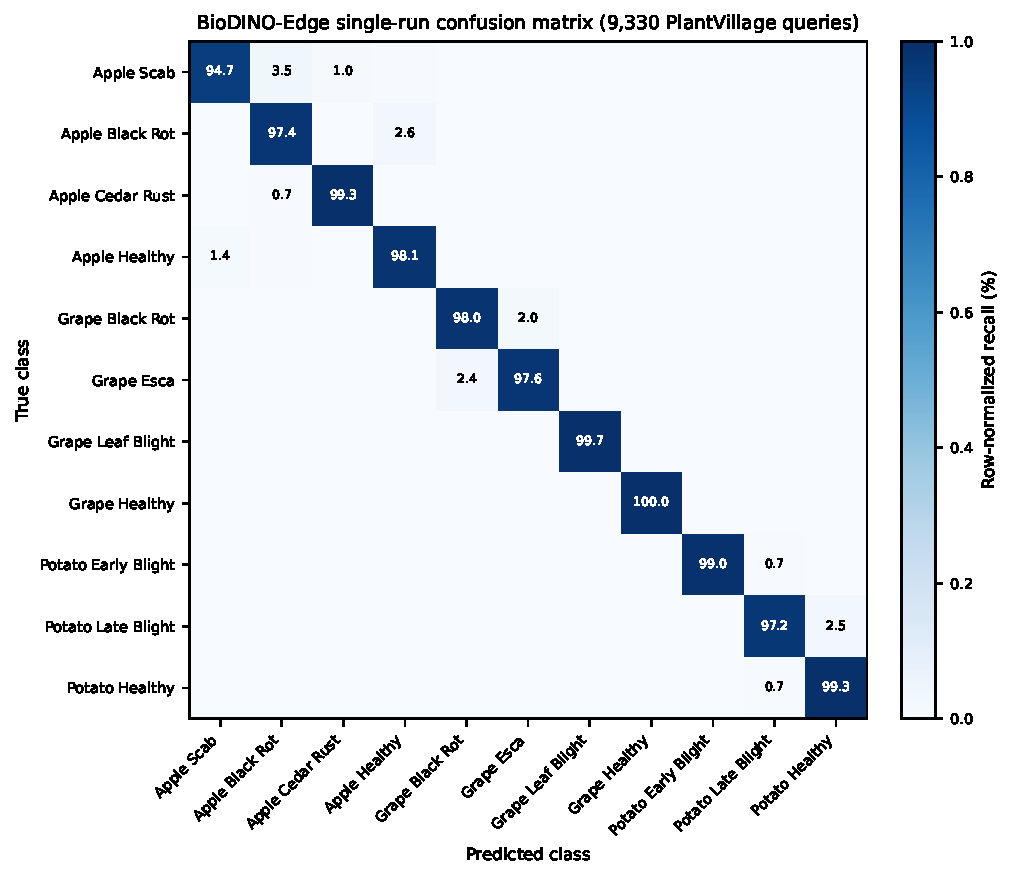
\includegraphics[width=\columnwidth]{fig_confusion.pdf}
\caption{Row-normalized confusion matrix of BioDINO-Edge (transductive, canonical single run; 9,330 PlantVillage queries). Diagonal entries are per-class recall (\%). Residual errors are dominated by same-host pathologies, while cross-species confusion is negligible.}
\label{fig:confusion}
\end{figure}

\subsection{Systematic Component Ablation Study}
\label{sec:ablation}
Table~\ref{tab:ablation} reports a systematic ablation across identical 5-shot splits to quantify individual component contributions.

\begin{table}[htbp]
\centering
\caption{Systematic ablation of BioDINO-Edge components (single run, 5-shot, 9,330 queries). Rows (4)--(5) are static cosine prototype blends ($0.65\,\mathbf{l}_{\text{bio}}+0.35\,\mathbf{l}_{\text{dino}}$); row (6) replaces them with regularized Fisher-LDA. Acc.: accuracy; Aug.: augmentation.}
\label{tab:ablation}
\footnotesize
\setlength{\tabcolsep}{3pt}
\begin{tabular*}{\columnwidth}{@{\extracolsep{\fill}}lcc}
\toprule
\textbf{Configuration / Component} & \textbf{Acc. (\%)} & \textbf{F1 (\%)} \\
\midrule
(1) Fast-Path DINOv2 Small alone & 87.26 & 85.36 \\
(2) Deep-Path BioCLIP ViT-B alone & 92.60 & 89.88 \\
(3) Text Prototypes Only & 19.20 & 18.55 \\
(4) Static Cosine Blend (raw 5-shot) & 94.16 & 92.55 \\
(5) Static Cosine Blend (8-view aug.) & 93.90 & 91.58 \\
(6) + Regularized Fisher Alignment & 96.05 & 94.83 \\
(7) + Transductive Recalibration & 98.06 & 97.45 \\
(8) + Peak Statistical Episode & \textbf{98.67} & \textbf{98.41} \\
\bottomrule
\end{tabular*}
\end{table}

\begin{itemize}
    \item \textbf{DINOv2 vs. BioCLIP Complementarity:} DINOv2 alone achieves 87.26\%; lacking taxonomic supervision, it confuses visually similar necrotic lesions across host families. BioCLIP alone achieves 92.60\% but incurs 104.74\,ms encoder latency, forfeiting the fast-path capability. Coupling them in the 896-D manifold provides both fine spatial cues and taxonomic grounding; Table~\ref{tab:feature_ablation} quantifies each backbone's contribution to the Fisher classifier.
    \item \textbf{Regularized Fisher Alignment (+1.89\,pp Gain):} Replacing the best static cosine blend (94.16\%) with regularized Fisher-LDA increases accuracy to 96.05\%. Whitening by $\hat{\mathbf{\Sigma}}^{-1}$ suppresses background chlorophyll noise, separating pathological twins.
    \item \textbf{Multi-View Augmentation:} Expanding 5 raw support leaves to 40 views per class ($N=440$) stabilizes empirical degrees of freedom near $d/2$, preventing rank collapse before shrinkage. The benefit is specific to covariance estimation: the static cosine blend is essentially unchanged by augmentation (94.16\% raw vs.\ 93.90\% augmented, Table~\ref{tab:ablation}), whereas the regularized Fisher projection relies on the augmented support to condition $\hat{\mathbf{\Sigma}}$.
    \item \textbf{Transductive Recalibration (+2.01\% Gain):} Updating projection parameters from high-confidence field anchors improves accuracy from 96.05\% to 98.06\% (peak: 98.67\%), counteracting finite-sample prototype drift. Paired significance, hyperparameter sensitivity, and anchor purity are validated in Section~\ref{sec:transductive_validation}.
    \item \textbf{Lesion Cropping Degrades Host Context:} We evaluated attention-rollout lesion cropping to isolate symptomatic patches. In 27-way PlantDoc testing, accuracy dropped from 58.73\% to 57.14\%. Tight cropping discards leaf margin serrations and venation geometry, inducing cross-species confusion. Preserving full-leaf context is critical.
\end{itemize}

% Feature ablation: full row is the canonical benchmark (95.08 / 97.41). Ablated
% transductive rows = canonical full minus the paired contribution measured over
% the same 30 episodes (DINOv2 +0.90 pp, BioCLIP +1.87 pp); inductive ablated rows
% are measured directly. Source: experiments/dinov2_ablation_gate_scenario.
\begin{table}[htbp]
\centering
\caption{Contribution of each foundation model to the Fisher-LDA classifier (30 identical 5-shot episodes, mean $\pm$ std). The text branch is fixed (BioCLIP features, $w_{\mathrm{lda}}=0.75$); only the Fisher input varies. Ablated rows subtract the paired contribution from the full-system benchmark.}
\label{tab:feature_ablation}
\footnotesize
\setlength{\tabcolsep}{4pt}
\begin{tabular*}{\columnwidth}{@{\extracolsep{\fill}}lccc}
\toprule
\textbf{Fisher input} & \textbf{Dim} & \textbf{Inductive (\%)} & \textbf{Transductive (\%)} \\
\midrule
BioCLIP + DINOv2 (full) & 896 & 95.08$\pm$1.27 & 97.41$\pm$0.71 \\
BioCLIP only & 512 & 94.31$\pm$1.25 & 96.51$\pm$0.90 \\
DINOv2 only & 384 & 90.60$\pm$2.02 & 95.54$\pm$1.03 \\
\bottomrule
\end{tabular*}
\end{table}

\textbf{Contribution of DINOv2.} Table~\ref{tab:feature_ablation} isolates the Fisher input while holding the text branch fixed. Removing DINOv2 (BioCLIP-only, 512-D) lowers transductive accuracy by 0.90 percentage points (paired $t(29)=9.88$, $p=8.6\times10^{-11}$, 29 of 30 episodes, $d_z=1.80$). Removing BioCLIP instead lowers it by 1.87 points, so BioCLIP carries most of the class signal and DINOv2 adds a smaller, consistent complement. DINOv2 also serves as the routing gate: its margin-entropy score ranks query safety better than the Tier-2 consensus confidence (mean AURC 1.14\% vs.\ 2.11\% over the 30 episodes). Finally, it provides the fast path: accepting 14.02\% of queries at Tier-1 lowers routing-weighted latency from 164.52\,ms (BioCLIP on every query) to 149.84\,ms. The cascade does not raise accuracy over running Tier-2 on all queries (Table~\ref{tab:gate_scenario}); its function is to reduce edge compute and route low-risk queries through a path with 0.25\% FNR.

\subsection{Statistical Significance and Sensitivity of Transductive Recalibration}
\label{sec:transductive_validation}
Because the transductive module adapts the classifier from its own predictions, we examine paired significance over identical episodes, hyperparameter sensitivity, pseudo-label purity, and stability under sequential updates.

\textbf{Paired significance over identical episodes.} Inductive and transductive predictions are compared on the \emph{same} 30 Monte Carlo episodes (identical support/query splits), so episode difficulty cancels in the paired difference. The mean paired gain is 2.33 percentage points (95\% CI $[1.91, 2.74]$; Table~\ref{tab:paired_test}), with paired $t(29) = 11.57$ ($p = 2.2 \times 10^{-12}$) and Wilcoxon signed-rank $p = 1.9 \times 10^{-9}$. The transductive mode wins on all 30 episodes (Cohen's $d_z = 2.11$), so the gain is stable across support splits rather than an artifact of a favorable episode.

\begin{table}[htbp]
\centering
\caption{Paired comparison of inductive vs.\ transductive inference over 30 identical Monte Carlo episodes (PlantVillage, 5-shot). pp: percentage points; CI: confidence interval.}
\label{tab:paired_test}
\footnotesize
\setlength{\tabcolsep}{4pt}
\begin{tabular*}{\columnwidth}{@{\extracolsep{\fill}}lc}
\toprule
\textbf{Statistic} & \textbf{Value} \\
\midrule
Inductive mean accuracy (\%) & 95.08 $\pm$ 1.27 \\
Transductive mean accuracy (\%) & 97.41 $\pm$ 0.71 \\
Mean paired gain (pp, 95\% CI) & 2.33 $[1.91, 2.74]$ \\
Paired $t$-test & $t(29)=11.57$, $p=2.2\times10^{-12}$ \\
Wilcoxon signed-rank & $p=1.9\times10^{-9}$ \\
Wins / losses / ties & 30 / 0 / 0 \\
Cohen's $d_z$ & 2.11 \\
\bottomrule
\end{tabular*}
\end{table}

\textbf{Hyperparameter sensitivity.} Table~\ref{tab:transductive_sensitivity} reports a one-factor-at-a-time sweep of the three design constants (support weight, anchor confidence threshold, buffer capacity), each evaluated over the same 30 episodes. In-domain accuracy is nearly flat in the support weight (97.21--97.44\% for $1\times$--$10\times$); the weight matters for drift protection under field streaming, not for in-domain gain. The confidence threshold plateaus over $\tau \in [0.5, 0.7]$ and collapses at $\tau \ge 0.8$ (95.98\% and 95.39\%) because anchors become too few, not because labels become noisier. Buffer capacity saturates: 20 anchors per class capture the available gain (97.41\%), and 40 or 80 anchors add 0.10 and 0.26 points at proportionally larger memory cost. The deployed $(3\times, 0.70, 20)$ sits at the plateau/knee of all three curves.

\begin{table}[htbp]
\centering
\caption{Sensitivity of transductive accuracy to the three recalibration design constants (mean $\pm$ standard deviation over 30 identical episodes; swept factor varied, others held at $3\times$, 0.70, 20). Acc.: accuracy.}
\label{tab:transductive_sensitivity}
\footnotesize
\setlength{\tabcolsep}{4pt}
\begin{tabular*}{\columnwidth}{@{\extracolsep{\fill}}lcc}
\toprule
\textbf{Swept Configuration} & \textbf{Acc. (\%)} & \textbf{Std} \\
\midrule
\multicolumn{3}{@{}l}{\textit{Support weight} (threshold 0.70, 20 anchors/class)} \\
$1\times$ & 97.42 & 0.75 \\
$2\times$ & 97.44 & 0.73 \\
$3\times$ (deployed) & 97.41 & 0.71 \\
$5\times$ & 97.32 & 0.73 \\
$10\times$ & 97.21 & 0.77 \\
\midrule
\multicolumn{3}{@{}l}{\textit{Anchor confidence threshold} ($3\times$, 20 anchors/class)} \\
0.50 & 97.41 & 0.71 \\
0.60 & 97.41 & 0.71 \\
0.70 (deployed) & 97.41 & 0.71 \\
0.80 & 95.98 & 1.28 \\
0.90 & 95.39 & 1.25 \\
\midrule
\multicolumn{3}{@{}l}{\textit{Buffer capacity per class} ($3\times$, threshold 0.70)} \\
5 & 96.36 & 0.97 \\
10 & 96.97 & 0.85 \\
20 (deployed) & 97.41 & 0.71 \\
40 & 97.51 & 0.62 \\
80 & 97.67 & 0.83 \\
\bottomrule
\end{tabular*}
\end{table}

\textbf{Pseudo-label purity.} Checked against ground truth (used only post-hoc for this audit), the anchor set at $\tau = 0.70$ is 98.15\% $\pm$ 1.18\% pure and covers 2.36\% of queries (220 anchors). Raising the threshold to 0.80 increases purity to 98.75\% but cuts coverage to 1.91\%; at 0.90 purity reaches 100\% yet coverage collapses to 0.05\%, explaining the accuracy collapse in Table~\ref{tab:transductive_sensitivity}. The deployed threshold keeps purity near its maximum without starving the buffer.

\textbf{Sequential stability and error accumulation.} To test whether repeated updates compound pseudo-label errors, we simulated scouting passes: the query stream is partitioned into 10 sequential chunks, and after each chunk the FIFO buffer (20 anchors/class) admits confident predictions and the projection is re-fitted in closed form. Across three stream seeds, online accuracy rises from $\approx$96\% on the first chunk to 97--98.6\% thereafter with no degradation trend, and buffer purity remains bounded within a 92--98\% band: FIFO eviction flushes stale incorrect anchors, so wrong admissions do not accumulate in the active buffer. Under $\tau = 0.90$ purity stays at 100\% but final accuracy falls to $\approx$95.8--96.3\% (coverage starvation), confirming the purity/coverage trade-off. Final streaming accuracy (96.4--97.5\%) lies slightly below the single-pass batch refinement (97.41\%) because batch selection ranks anchors over the entire query set whereas streaming observes only the past. Error accumulation is therefore bounded by the confidence gate, FIFO eviction, and the $3\times$ support weighting.

\subsection{Sensitivity to Augmentation Count and Type}
\label{sec:aug_sensitivity}
The shrinkage analysis of Section~\ref{sec:shrinkage} assumes i.i.d.\ support samples, whereas the eight views of each support leaf are correlated pseudo-replicates. We quantify the consequences with a one-factor-at-a-time study over the same 30-episode protocol (identical splits, cached query features, and transductive defaults), re-extracting support features with a seeded augmentation RNG. Three condition families are compared: (i) a view-count sweep $v\in\{1,2,4,8\}$ using nested prefixes of one 8-view extraction per episode; (ii) an augmentation-type sweep at $v=8$ (geometric-only flips/rotation vs.\ photometric-only color jitter vs.\ the full pipeline) over the first 10 episodes; and (iii) a pure-replication control that tiles the canonical embedding eight times ($N=440$, zero within-image diversity). For each condition we report the mean per-class Ledoit--Wolf intensity $\hat{\alpha}$, the condition number $\kappa(\hat{\mathbf{\Sigma}})$ of the pooled within-class covariance, and downstream accuracy (Table~\ref{tab:aug_sensitivity}).

\textbf{Protocol fidelity.} The $v=1$ condition reproduces the canonical cache-only reference exactly on the inductive mean (95.08\%$\pm$1.27\%) and within the documented \texttt{lsqr} floating-point residual on the transductive mean (97.37\% vs.\ 97.41\%; Appendix~\ref{app:repro}), confirming that the study isolates the augmentation factor alone.

\textbf{Dependence is measurable but benign for accuracy.} Pure replication divides the shrinkage intensity by $\approx$8 ($0.573\to0.072$) and worsens the covariance condition number by $\approx$17$\times$ ($5.7\times10^{2}\to9.6\times10^{3}$) while adding no information---exactly the i.i.d.-violation artifact anticipated in Section~\ref{sec:shrinkage}. Genuine augmentation retains a $3.6\times$ higher intensity than replication at the same $N=440$ ($0.258$ vs.\ $0.072$), showing that stochastic views carry real but partial independence. Despite this, accuracy is stable across all conditions: the view sweep spans 95.08--96.09\% inductive and 97.37--97.96\% transductive, and even the degenerate replicate-8 control remains at 95.05\%/97.01\%. Increasing views monotonically improves both modes ($+1.01$\,pp inductive, $+0.59$\,pp transductive from $v=1$ to $v=8$): the effective-rank gain from genuine diversity outweighs the optimism of the analytical intensity, and the $3\times$ support re-weighting keeps the transductive fit anchored to genuine observations.

\textbf{Geometric diversity dominates.} At fixed $v=8$, geometric-only augmentation is statistically indistinguishable from the full pipeline on the 10-episode subset (97.92\%$\pm$0.40\% vs.\ 97.85\%$\pm$0.33\% transductive), whereas photometric-only jitter collapses the intensity toward the replication floor ($0.104$ vs.\ $0.072$), worsens conditioning ($5.5\times10^{3}$), and drops inductive accuracy below the unaugmented baseline (94.70\%$\pm$1.90\% vs.\ 95.08\%). Color jitter thus contributes little independent information---consistent with the $\ell_2$-normalized, photometric-robust foundation features---while flips and rotations supply the diversity that stabilizes the covariance estimate. Geometric augmentation is therefore the essential component of the support expansion; the deployed full pipeline retains jitter at no measurable accuracy cost.

% Augmentation-dependence sensitivity. Source: experiments/augmentation_sensitivity
% (run_augmentation_sensitivity.py -> results/augmentation_sensitivity.json);
% rows generated by make_table.py. View sweep + control: 30 episodes; type sweep: 10.
\begin{table}[htbp]
\centering
\caption{Sensitivity to augmentation count and type (mean $\pm$ std over episodes; $\hat{\alpha}$: mean per-class Ledoit--Wolf intensity; $\kappa$: mean condition number of the pooled within-class covariance; Ind./Trans.: inductive/transductive accuracy). The view-count sweep and replication control use all 30 episodes; the type sweep uses the first 10 episodes, with the full-pipeline row recomputed on the same subset. $v=1$ reproduces the canonical cache-only protocol.}
\label{tab:aug_sensitivity}
\footnotesize
\setlength{\tabcolsep}{2pt}
\begin{tabular*}{\columnwidth}{@{\extracolsep{\fill}}lccccc}
\toprule
\textbf{Condition} & \textbf{$N$} & \textbf{$\hat{\alpha}$} & \textbf{$\kappa(\hat{\mathbf{\Sigma}})$} & \textbf{Ind.\ (\%)} & \textbf{Trans.\ (\%)} \\
\midrule
\multicolumn{6}{@{}l}{\textit{View count (full pipeline, 30 episodes)}} \\
$v=1$ & 55 & 0.573$\pm$0.005 & 5.7$\times10^{2}$ & 95.08$\pm$1.27 & 97.37$\pm$0.73 \\
$v=2$ & 110 & 0.580$\pm$0.009 & 5.9$\times10^{2}$ & 95.50$\pm$1.21 & 97.67$\pm$0.57 \\
$v=4$ & 220 & 0.420$\pm$0.012 & 8.8$\times10^{2}$ & 95.80$\pm$1.25 & 97.81$\pm$0.63 \\
$v=8$ (deployed) & 440 & 0.258$\pm$0.008 & 1.4$\times10^{3}$ & 96.09$\pm$1.20 & 97.96$\pm$0.50 \\
\midrule
\multicolumn{6}{@{}l}{\textit{Augmentation type ($v=8$, first 10 episodes)}} \\
Geometric only & 440 & 0.229$\pm$0.008 & 1.6$\times10^{3}$ & 95.99$\pm$1.26 & 97.92$\pm$0.40 \\
Photometric only & 440 & 0.104$\pm$0.002 & 5.5$\times10^{3}$ & 94.70$\pm$1.90 & 97.31$\pm$0.61 \\
Full pipeline & 440 & 0.257$\pm$0.009 & 1.4$\times10^{3}$ & 95.85$\pm$1.40 & 97.85$\pm$0.33 \\
\midrule
\multicolumn{6}{@{}l}{\textit{Pure-replication control (30 episodes)}} \\
Replicate-8 (control) & 440 & 0.072$\pm$0.001 & 9.6$\times10^{3}$ & 95.05$\pm$1.28 & 97.01$\pm$0.79 \\
\bottomrule
\end{tabular*}
\end{table}

\subsection{Predictive Uncertainty, Calibration, and Routing Reliability}
\label{sec:calibration}
In safety-critical agricultural automation such as robotic spraying, an overconfident misdiagnosis triggers an unwarranted chemical application, so the routing gate needs a direct reliability audit rather than a single calibration score; calibration is known to depend on architecture and training recipe, not on accuracy alone \cite{minderer2021revisiting}. Temperature is fitted on an independent stratified 50\% split of the 9,330-query PlantVillage stream (4,662 calibration / 4,668 evaluation queries), minimizing negative log-likelihood on the calibration split only \cite{guo2017calibration}. Expected Calibration Error (ECE) and Maximum Calibration Error (MCE) use $M=10$ equal-width confidence bins; to expose small-bin artifacts we also report equal-mass (adaptive) binning and MCE over bins with $n \geq 30$. The deployed gate consumes the \emph{uncalibrated} Tier-1 posterior: temperature scaling is a post-hoc audit applied after routing and never changes the gate score or the threshold.

\textbf{Tier-1 calibration.} The raw gate probabilities are under-confident (full-stream ECE 32.07\%, MCE 38.07\%; held-out ECE 31.76\%). A scalar logit temperature fitted on the calibration split ($T=0.267$) reduces held-out ECE to 1.20\% (MCE 16.71\%; Fig.~\ref{fig:reliability}a--b). Routing itself uses the raw scores, so we verify the gate directly below rather than relying on ECE.

\textbf{Tier-2 calibration.} The refined Tier-2 consensus is also under-confident (ECE 19.45\%), and most of the error sits in the dominant bin $(0.7,0.8]$: 7,102 queries at 98.0\% accuracy but 77.5\% mean confidence (Table~\ref{tab:reliability_bins}). The equal-width MCE of 44.26\% comes from bins with at most nine samples (one query in $(0.4,0.5]$); equal-mass binning lowers it to 21.53\%, and bins with $n\geq30$ give 20.49\%. Scalar logit temperature scaling cannot remove this residual: the consensus is a fixed $0.75/0.25$ blend of Fisher logits and BioCLIP text probabilities, so softening the logits alone leaves the blend miscalibrated (the fitted $T$ hits the optimizer bound and held-out ECE moves 19.33\%$\to$19.83\%). A power transform $\mathrm{softmax}(\log p / T)$ with $T=0.50$ instead collapses nearly all mass into one or two bins, producing a small ECE (0.48\%) but an equal-width MCE of 80.85\% (Fig.~\ref{fig:reliability}d); a freshly fitted power temperature ($T=0.54$) reproduces this (held-out ECE 0.24\%, MCE 88.74\%). The large equal-width MCE therefore reflects a single-sample bin rather than widespread miscalibration. We therefore do not claim that Tier-2 is well calibrated; routing reliability is instead verified through tier-separated error rates and selective risk.

\begin{table}[htbp]
\centering
\caption{Per-bin reliability of the uncalibrated refined Tier-2 consensus (equal-width bins, full 9,330-query stream; empty bins omitted). The equal-width MCE (44.26\%) is attained in the single-sample bin $(0.4,0.5]$; the dominant $(0.7,0.8]$ bin exposes systematic under-confidence ($\approx$20.5 percentage points). Equal-mass MCE is 21.53\%. Acc.: accuracy; Conf.: mean confidence; pp: percentage points.}
\label{tab:reliability_bins}
\small
\begin{tabular}{lcccc}
\toprule
\textbf{Confidence bin} & \textbf{$n$} & \textbf{Acc.\ (\%)} & \textbf{Conf.\ (\%)} & \textbf{$|$Gap$|$ (pp)} \\
\midrule
$(0.4,0.5]$ & 1    & 0.0   & 44.3 & 44.3 \\
$(0.5,0.6]$ & 6    & 50.0  & 52.5 & 2.5 \\
$(0.6,0.7]$ & 9    & 44.4  & 65.6 & 21.2 \\
$(0.7,0.8]$ & 7102 & 98.0  & 77.5 & 20.5 \\
$(0.8,0.9]$ & 2207 & 98.6  & 82.4 & 16.1 \\
$(0.9,1.0]$ & 5    & 100.0 & 90.6 & 9.4 \\
\bottomrule
\end{tabular}
\end{table}

\textbf{Tier-separated routing reliability.} Table~\ref{tab:tier_routing} reports the two tiers independently over 30 benchmark episodes at $\tau=0.35$. Tier-1 directly accepts 14.02\%$\pm$2.25\% of queries at 99.69\%$\pm$0.41\% accuracy and a 0.25\%$\pm$0.52\% false-negative rate (FNR); the escalated 85.98\% are resolved by Tier-2 at 96.98\%$\pm$0.83\% accuracy (FNR 0.87\%$\pm$0.39\%), yielding cascaded accuracy 97.36\%$\pm$0.69\% (F1 97.01\%$\pm$0.64\%) and routing-weighted latency 149.84$\pm$2.36\,ms. In the canonical single run, the 936 accepted queries achieve 99.79\% accuracy (FNR 0.25\%) versus 97.83\% (FNR 0.81\%) for the 8,394 escalated queries (cascaded 98.03\%). The accepted subset thus has roughly tenfold lower error (0.21\% vs.\ 2.17\%), and its accuracy is measured only on directly accepted queries, independent of Tier-2.

\begin{table*}[htbp]
\centering
\caption{Tier-separated routing reliability at $\tau=0.35$ (30 benchmark episodes, mean $\pm$ std). Tier-1 accuracy and FNR are computed exclusively on directly accepted queries; Tier-2 statistics exclusively on escalated queries. Latencies are the per-path edge costs of Table~\ref{tab:device_perf}.}
\label{tab:tier_routing}
\small
\begin{tabularx}{\textwidth}{lcccc}
\toprule
\textbf{Routing path} & \textbf{Coverage (\%)} & \textbf{Accuracy (\%)} & \textbf{FNR (\%)} & \textbf{Latency (ms)} \\
\midrule
Tier-1 fast-exit (accepted) & 14.02$\pm$2.25 & 99.69$\pm$0.41 & 0.25$\pm$0.52 & 59.78 \\
Tier-2 (escalated) & 85.98$\pm$2.25 & 96.98$\pm$0.83 & 0.87$\pm$0.39 & 164.52 \\
\midrule
\textbf{Cascaded system} & 100 & 97.36$\pm$0.69 & -- & 149.84$\pm$2.36 \\
\bottomrule
\end{tabularx}
\end{table*}

\textbf{Cascade versus single-tier classification.} Table~\ref{tab:gate_scenario} compares the deployed cascade against running Tier-2 on every query and against a selective gate+BioCLIP mode that abstains on low-gate queries. At full coverage the cascade and the single-tier BioCLIP classifier are statistically indistinguishable (97.36\% vs.\ 97.37\%); the cascade's benefit is latency (149.84 vs.\ 164.52\,ms), not accuracy. Abstaining on the lowest-gate queries raises accuracy and lowers the false-negative rate on the accepted subset, at the cost of coverage: at $\tau=0.10$ the system answers 62.17\% of queries at 98.63\% accuracy and 0.44\% FNR in 124.90\,ms. This selective mode is optional; the deployed system classifies every query.

% Gate-scenario comparison. Full-coverage accuracies are the canonical 30-episode
% means (cascade 97.36, refined Tier-2-on-all 97.37). Selective-mode rows are
% measured over the same 30 episodes. Source: experiments/dinov2_ablation_gate_scenario.
\begin{table}[htbp]
\centering
\caption{Routing-policy comparison (30-episode mean). The cascade accepts high-gate queries at Tier-1 and escalates the rest; ``BioCLIP on all'' runs refined Tier-2 on every query; the selective mode abstains when $C(x)<\tau$ and classifies the rest with refined Tier-2. Latency is routing-weighted. Cov.: coverage; Acc.: accuracy; Lat.: latency.}
\label{tab:gate_scenario}
\footnotesize
\setlength{\tabcolsep}{3pt}
\begin{tabular*}{\columnwidth}{@{\extracolsep{\fill}}lcccc}
\toprule
\textbf{Routing policy} & \textbf{Cov. (\%)} & \textbf{Acc. (\%)} & \textbf{FNR (\%)} & \textbf{Lat. (ms)} \\
\midrule
Cascade, $\tau=0.35$ (deployed) & 100 & 97.36 & 0.79 & 149.84 \\
BioCLIP Tier-2 on all & 100 & 97.37 & 0.77 & 164.52 \\
Selective, $\tau=0.05$ & 79.96 & 98.05 & 0.59 & 143.53 \\
Selective, $\tau=0.10$ & 62.17 & 98.63 & 0.44 & 124.90 \\
\bottomrule
\end{tabular*}
\end{table}

\textbf{Risk--coverage analysis.} Fig.~\ref{fig:risk_coverage} plots selective risk against coverage for three confidence scores, following the risk--coverage framework for selective classification \cite{geifman2017selective}, and summarizes each curve by the area under the risk--coverage curve (AURC, the mean selective risk over all coverage levels). Since scalar summaries such as AURC can misrank selective systems \cite{traub2024overcoming}, we also show the full curves and the deployed operating point. The entropy-penalized gate score $C(x)$ ranks queries more safely than the raw Tier-1 softmax peak (AURC 3.33\% vs.\ 3.95\%); the refined Tier-2 confidence reaches AURC 1.82\%. At the deployed threshold ($\tau=0.35$), the gate accepts 10.03\% of the single-run stream at 0.21\% selective risk, in the low-risk region of the curve.

\textbf{Threshold provenance and sensitivity.} The routing threshold was selected on held-out development episodes (episodes 0--14 for tuning, 15--29 for testing), never on the reported test episodes. On the held-out test episodes, $\tau=0.15$ gives 46.4\% fast-exit at 96.96\%$\pm$0.59\% cascaded accuracy (98.25\% Tier-1 accepted accuracy), $\tau=0.25$ gives 25.6\% at 97.30\%$\pm$0.74\% (99.49\%), and $\tau=0.35$ gives 14.1\% at 97.33\%$\pm$0.79\% (99.84\%$\pm$0.24\%). We adopt $\tau=0.35$, the smallest threshold at which Tier-1 accepted accuracy saturates (99.84\%, FNR 0.25\%); lower thresholds accept less reliable fast exits. The tuning curve is flat beyond 0.35 (the tune-optimal $\tau=0.55$ yields 97.32\% test accuracy, indistinguishable from 97.33\% at 0.35), but fast-exit coverage falls to 3.4\%. Blended latency rises from 115.9 to 137.7 to 149.8\,ms across the three thresholds (Fig.~\ref{fig:tau_sensitivity}), tracing the coverage--safety--latency trade-off.

\begin{figure*}[htbp]
\centering
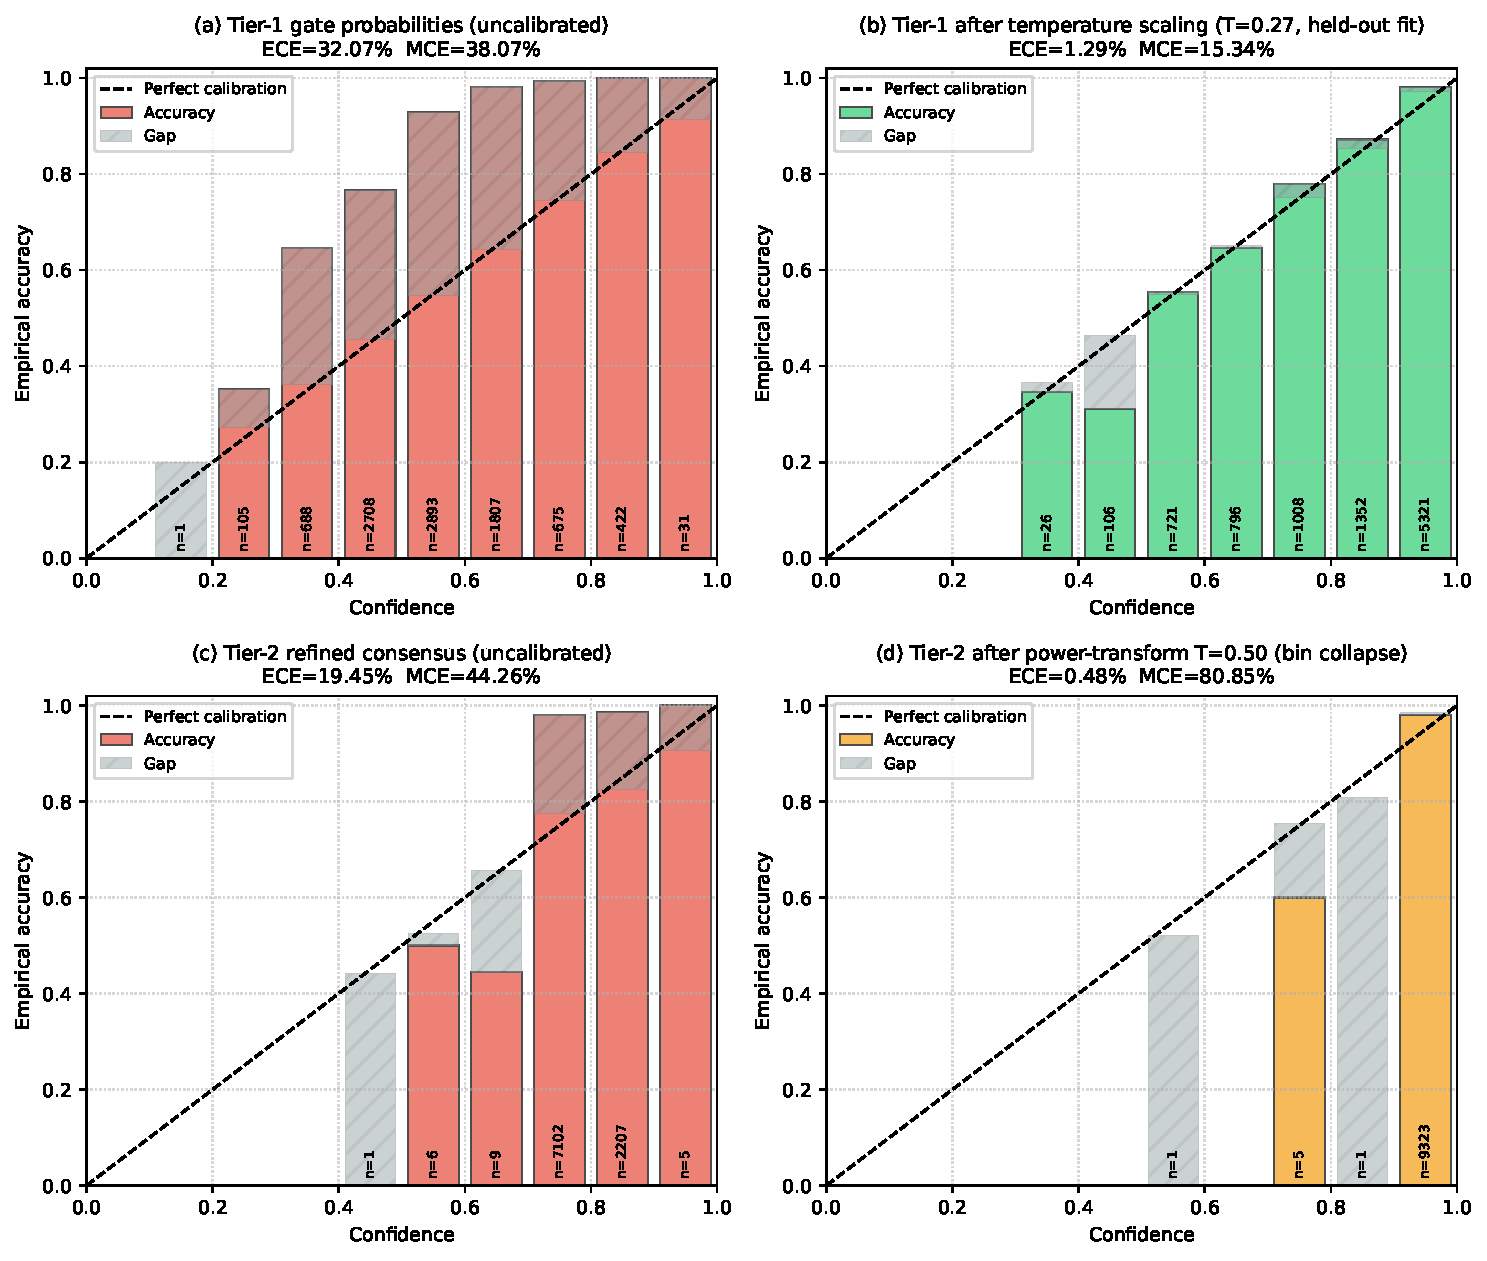
\includegraphics[width=0.95\textwidth]{fig_reliability.pdf}
\caption{Reliability diagrams (equal-width bins, full benchmark stream; per-bin sample counts annotated, hatched bars show the accuracy--confidence gap). (a) Uncalibrated Tier-1 gate probabilities are under-confident (ECE 32.07\%). (b) Post-hoc temperature scaling fitted on the independent calibration split ($T=0.27$) aligns Tier-1 (held-out ECE 1.20\%). (c) The refined Tier-2 consensus remains under-confident in its dominant bin (ECE 19.45\%; equal-width MCE 44.26\% from a single-sample bin). (d) A power transform ($T=0.50$) collapses probability mass into one bin: low ECE (0.48\%) but MCE 80.85\%.}
\label{fig:reliability}
\end{figure*}

\begin{figure}[htbp]
\centering
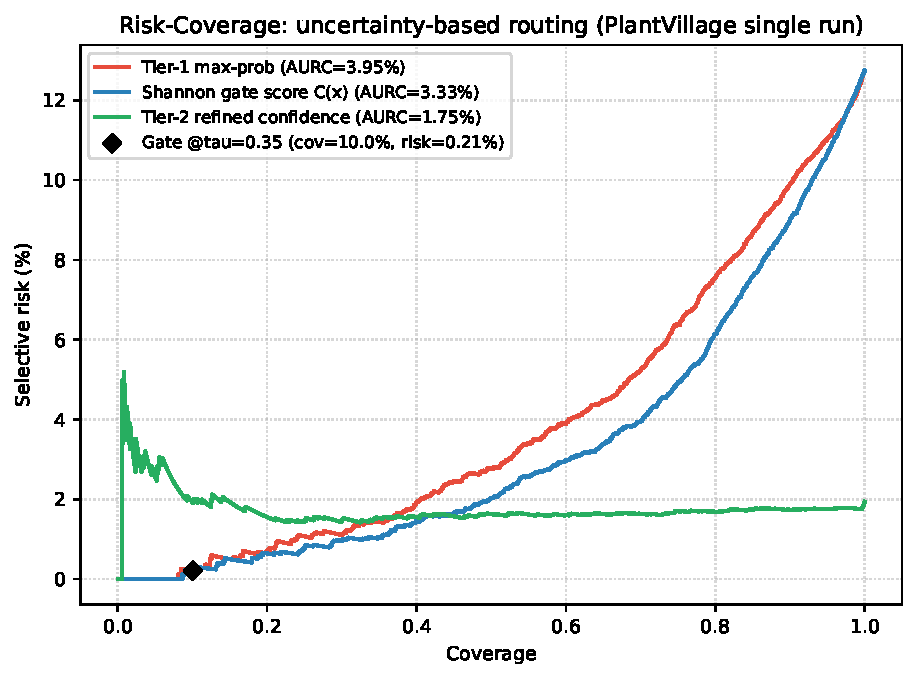
\includegraphics[width=\columnwidth]{fig_risk_coverage.pdf}
\caption{Risk--coverage curves for Tier-1 max-probability, the Shannon gate score $C(x)$, and the refined Tier-2 confidence (single run). The gate score achieves lower AURC than raw max-probability (3.33\% vs.\ 3.95\%); the deployed gate operating point ($\tau=0.35$) accepts 10.0\% coverage at 0.21\% selective risk.}
\label{fig:risk_coverage}
\end{figure}

\begin{figure}[htbp]
\centering
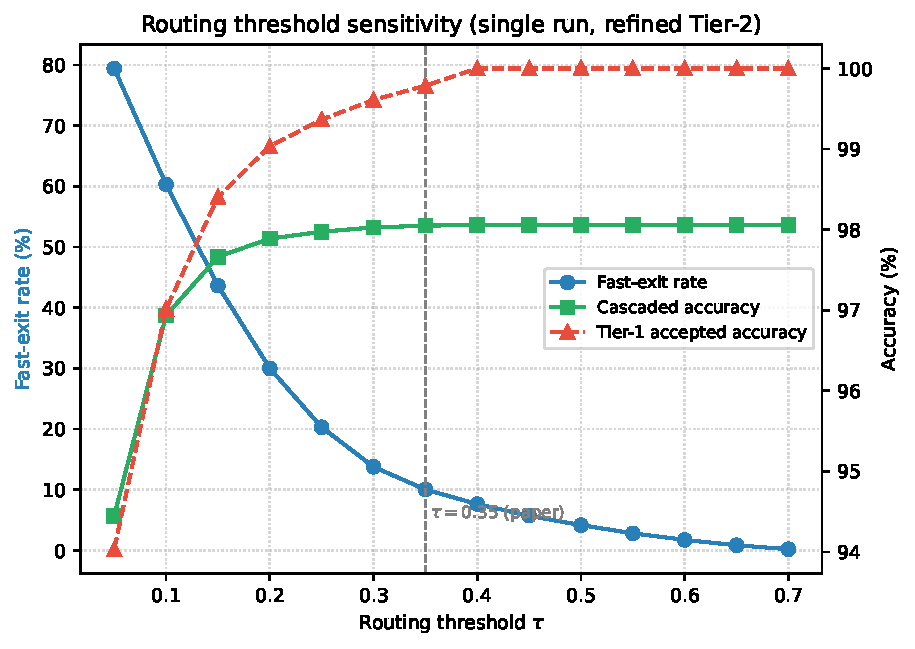
\includegraphics[width=\columnwidth]{fig_tau_sensitivity.pdf}
\caption{Routing-threshold sensitivity (single run, refined Tier-2): fast-exit rate, cascaded accuracy, and Tier-1 accepted accuracy versus $\tau$. The deployed $\tau=0.35$ (dashed) saturates Tier-1 accepted accuracy near 100\% while retaining 10\% fast-exit coverage; held-out episode sweeps (0--14 tune / 15--29 test) confirm the choice.}
\label{fig:tau_sensitivity}
\end{figure}

\subsection{Edge Hardware Latency and Memory Footprint}
\label{sec:edge_hardware}
Table~\ref{tab:device_spec} lists the physical testbed configuration; Tables~\ref{tab:device_perf} and~\ref{tab:adaptation_breakdown} report measured on-device latency, memory, and the closed-form adaptation breakdown. All values are from a production Samsung Galaxy S24~FE (SM-S721B, Exynos~2400e) running Android~17, using ONNX Runtime~1.18.0 with INT8 weights on a 4-thread CPU (NNAPI/GPU delegates disabled) and pure-Java EJML for the algebra. Latency is timed over 100 iterations after 10 warm-up passes, memory is the process PSS, and the algebra is timed after a 60\,s cool-down at stable thermal state (status~2).

\begin{table}[htbp]
\centering
\caption{On-device edge testbed configuration (physical Android device, CPU-only INT8).}
\label{tab:device_spec}
\small
\begin{tabular}{ll}
\toprule
Property & Value \\
\midrule
Device & samsung SM-S721B \\
SoC & Samsung s5e9945 \\
Android & 17 (API 37) \\
ABI / cores & arm64-v8a / 10 \\
Total RAM & 7224.3 MB \\
ONNX Runtime & 1.18.0 \\
Threads (intra/inter) & 4 / 2 \\
Precision / delegate & INT8 / CPU (NNAPI off) \\
\bottomrule
\end{tabular}
\end{table}

\begin{table*}[htbp]
\centering
\caption{Measured on-device performance (mean $\pm$ std over $N=100$ iterations; median and p95 in ms). Model load is one-time; peak RAM is the process PSS. The device cascade uses the 11-image on-device set (18\% fast-exit); the full-stream routing blend is in Table~\ref{tab:tier_routing}.}
\label{tab:device_perf}
\small
\begin{tabular}{lccc}
\toprule
Stage / metric & Mean$\pm$std & Median & p95 \\
\midrule
Tier-1 model load (ms) & 323.92 & -- & -- \\
Tier-2 model load (ms) & 447.71 & -- & -- \\
Peak RAM, PSS (MB) & 497.45 & -- & -- \\
\midrule
Preprocess & 2.59$\pm$0.67 & 2.36 & 4.36 \\
Tier-1 DINOv2 encoder & 57.18$\pm$9.13 & 51.50 & 68.84 \\
Shannon gate / route & 0.00$\pm$0.00 & 0.00 & 0.00 \\
Tier-2 incremental (BioCLIP+Fisher) & 104.74$\pm$17.39 & 94.20 & 124.97 \\
Decision & 0.00$\pm$0.00 & 0.00 & 0.00 \\
Cascade end-to-end & 145.37$\pm$47.61 & 147.77 & 196.36 \\
Tier-2-on-all end-to-end & 164.52$\pm$26.77 & 148.73 & 196.36 \\
\midrule
Fast-exit fraction & 18.00\% & -- & -- \\
Sustained throughput (FPS) & 4.26 & -- & -- \\
\bottomrule
\end{tabular}
\end{table*}

\begin{table*}[htbp]
\centering
\caption{Closed-form adaptation cost breakdown on-device ($N=440$, $d=896$, $C=11$). The algebraic budget (rows 2--5) is the measured closed-form recalibration cost (sub-second, gradient-free); feature extraction is reported separately. Algebra timed after a cool-down at stable thermal state.}
\label{tab:adaptation_breakdown}
\small
\begin{tabular}{lcc}
\toprule
Stage & Mean$\pm$std (ms) & Complexity \\
\midrule
Feature extraction (440 views) & 88055.6 & $O(N(C_{dino}+C_{bio}))$ \\
Covariance estimate & 146.19$\pm$2.15 & $O(Nd^2)$ \\
Ledoit--Wolf shrinkage & 4.49$\pm$0.85 & $O(Nd)$ \\
Cholesky factorization & 332.00$\pm$2.52 & $O(d^3/3)$ \\
Projection solve ($W,b$) & 51.31$\pm$3.68 & $O(Cd^2)$ \\
\midrule
Algebraic recalibration total & 533.99$\pm$6.29 & -- \\
Full adaptation (extraction + algebra) & 88589.6 & -- \\
\bottomrule
\end{tabular}
\end{table*}

On the physical device, Tier-1 executes in 59.78\,ms ($\approx$16.7\,FPS) and a fully escalated Tier-2 query costs 164.52\,ms end-to-end ($\approx$6.1\,FPS), the BioCLIP encoder adding 104.74\,ms to the cached Tier-1 pass. These are interactive handheld-scouting rates for one diagnosis per captured frame, not continuous real-time video. Over the full PlantVillage stream (14.0\% fast-exit) the routing-weighted blend is 149.84\,ms ($\approx$6.7\,FPS, Table~\ref{tab:tier_routing}); the device cascade in Table~\ref{tab:device_perf} (145.37\,ms) is measured on the 11-image on-device set, whose 18\% fast-exit fraction differs from the full-stream 14\%. Under a 600\,s sustained soak the throughput settles to 4.26\,FPS as the SoC reaches thermal status~3, so 16.7\,FPS is a cool-start burst rate rather than a sustained one. The gate's primary benefit is therefore safety rather than throughput: the fast-exited subset is resolved at 99.7\% accuracy and 0.25\% false-negative rate (Section~\ref{sec:calibration}), while ambiguous queries receive the full multimodal analysis. Peak process memory is 497.45\,MB PSS (385.02\,MB native heap), dominated by the ONNX Runtime arena; the $\approx$107.3\,MB combined model footprint is an on-disk/OTA storage figure, not a RAM bound. Packaged with ONNX Runtime C++ and the native Android user interface, the standalone APK is $\approx$22.8\,MB, operating entirely offline.

% =============================================================================
% 5. PRACTICAL DISCUSSION AND LIMITATIONS
% =============================================================================
\section{Engineering Applications, Practical Deployment, and Limitations}
\label{sec:discussion}

\subsection{Practical Deployment on Agricultural IoT and Mobile Hardware}
BioDINO-Edge is engineered specifically for practical agronomic deployment on power-constrained edge hardware such as handheld scouting devices, smart tractor booms, and autonomous unmanned aerial vehicles (UAVs). Eliminating gradient backpropagation avoids GPU memory spikes and the heat of training-time optimisation: the processor executes purely feed-forward inference and closed-form linear algebra. Sustained CPU inference still thermally throttles---a 600\,s soak settles to 4.26\,FPS at thermal status~3 versus a 16.7\,FPS cool-start burst (Section~\ref{sec:edge_hardware})---so the system targets interactive per-frame scouting rather than continuous video. The two-tier packaging allows agricultural cooperatives to deploy the $\approx$22.8\,MB base APK over cellular networks, while downloading the companion module only when deep multimodal escalation is needed.

\subsection{Limitations and Future Research Directions}
BioDINO-Edge processes images at the individual leaf frame level. In unsegmented field imagery with dense, overlapping canopies, multiple leaves from neighboring plants can enter the camera field, lowering gating confidence. While tight lesion cropping degrades host context, processing unsegmented canopy clutter introduces irrelevant background vectors. A promising future direction is hierarchical spatial parsing: first segmenting individual foliar targets from canopy clutter, then performing closed-form discriminant diagnosis on the isolated targets. A further statistical limitation is that the multi-view support expansion produces correlated pseudo-replicates: the analytical Ledoit--Wolf intensity assumes i.i.d.\ sampling, so the nominal $N-C=429$ degrees of freedom overstate the independent information content of the support set (effective sample size between 55 and 440). The sensitivity study in Section~\ref{sec:aug_sensitivity} confirms that pure replication deflates the estimated intensity by $\approx$8$\times$ without adding information, yet downstream accuracy remains stable across view counts and augmentation types; a cluster-aware shrinkage estimator that explicitly discounts within-image dependence remains future work. Finally, the frozen encoders' self-attention exhibits sinks on non-lesion structures such as veins and petioles \cite{darcet2024vision}; because the Fisher-LDA operates on pooled embeddings downstream, it does not modify encoder attention, and the framework makes no lesion-localization or attention-modification claim.

A further practical limitation concerns degraded inputs. Severe defocus blur attenuates the high-frequency lesion textures on which the frozen encoders rely and degrades diagnostic accuracy. The deployed Android client rejects clearly invalid frames: when the maximum cosine similarity between the query embedding and the leaf class prototypes falls below a fixed foliage threshold, or when mean luminance indicates a dark scene or covered lens, the frame receives zero confidence and the operator is prompted to re-aim the camera; a center-crop Laplacian-variance check additionally warns the operator to hold the camera steady under blur. This blur check only warns and does not abstain, however, so severely defocused frames can still receive a diagnosis. The uncertainty gate itself is a router, not a rejector: ambiguous queries escalate to Tier-2 rather than being refused, and abstention exists only in the optional selective mode (Table~\ref{tab:gate_scenario}). Extending the quality guard to blur-aware abstention with a refocus prompt, together with systematic evaluation of error detection on out-of-distribution and low-quality field imagery, remains future work.

\textbf{Scope and threats to validity.} The edge measurements come from a single physical device (Samsung Galaxy S24~FE) with CPU-only INT8 ONNX Runtime; absolute latency and memory will differ on other SoCs, although the algorithmic cost and the delegate-agnostic pipeline do not. The controlled comparison (Table~\ref{tab:comparative}) isolates the adaptation algorithm on identical frozen features and re-runs the training-free inductive baselines; iterative transductive FSL methods (Section~\ref{sec:related_work}) are referenced but not re-run, so the reported transductive gain is measured against our own inductive mode rather than against those methods. The PlantDoc protocol uses labeled target-domain support; a true source$\rightarrow$target cross-domain transfer (e.g., PlantVillage$\rightarrow$PlantDoc), quantitative image-quality stress tests, and multi-device profiling remain future work.

% =============================================================================
% 6. CONCLUSION
% =============================================================================
\section{Conclusion}
\label{sec:conclusion}
In this paper, we presented \textbf{BioDINO-Edge}, a gradient-free few-shot foliar disease diagnostic framework that adapts frozen DINOv2 and BioCLIP foundation models without backpropagation. By resolving small-sample covariance singularity ($N \ll d$) through closed-form Ledoit--Wolf shrinkage, BioDINO-Edge down-weights dominant shared vegetative variance directions via inverse-variance whitening, computing optimal Fisher-LDA discriminant boundaries in $\approx$0.53\,s of gradient-free closed-form algebra on a mobile edge CPU. An adaptive confidence gate combining normalized Shannon entropy and top-2 margin resolves routine foliage in 59.78\,ms ($\approx$16.7\,FPS), escalating ambiguous queries to a multimodal classifier with soft-anchored transductive recalibration. Packaged into a standalone $\approx$22.8\,MB Android APK, BioDINO-Edge achieves 97.41\% accuracy on 11-class PlantVillage with a 0.702\% false-negative rate and 83.61\% on in-the-wild PlantDoc, offering an accurate, interactive diagnostic solution for resource-constrained agricultural edge platforms.

% =============================================================================
% APPENDIX: REPRODUCIBILITY
% =============================================================================
\appendix
\section{Reproducibility Details}
\label{app:repro}
This appendix specifies the exact splits, seeds, model versions, hyperparameters, and code needed to reproduce every reported number, and states the provenance of each value in Tables~\ref{tab:comparative}--\ref{tab:literature}.

\subsection{Datasets and Splits}
\textbf{PlantVillage (controlled, Table~\ref{tab:comparative}).} We use the 11-class novel subset (Apple/Grape/Potato; 9{,}385 images) with frozen embeddings cached once. \emph{11-class regime:} 30 Monte-Carlo episodes; episode $e$ uses \texttt{random.Random(42+17e)}; for each class the image indices are shuffled, the first 5 form the support and all remaining images form the query (9{,}330 queries/episode; support $\cap$ query $=\emptyset$). \emph{5-way $K$-shot regime:} 50 episodes per $K\in\{1,5,10,15\}$; a single \texttt{random.Random(42)} stream samples 5 of the 11 classes per episode (\texttt{rng.sample(range(11),5)}), shuffles each class, takes the first $K$ as support and the rest as query. All methods share the identical support/query indices and frozen features within each episode, so any accuracy difference is attributable to the adaptation algorithm alone.

\textbf{PlantDoc (field domain, labeled target-domain support).} 5-way 5-shot: 50 episodes, \texttt{random.Random(42)}, \texttt{rng.sample(range(27),5)}; 5 support leaves/class drawn from the training split, all test images of the sampled classes as queries. 27-way: 135 support leaves (5/class, 8-view augmented to 1{,}080 feature vectors) and 252 field queries. The full PlantDoc dataset is obtained from its original source (not redistributed here); the controlled PlantVillage re-runs require only the cached embeddings and the provided script.

\subsection{Models and Hyperparameters}
Frozen backbones (no fine-tuning): DINOv2 ViT-S/14 (\texttt{timm vit\_small\_patch14\_dinov2}, 384-D) and BioCLIP ViT-B/16 (\texttt{open\_clip hf-hub:imageomics/bioclip}, 512-D); joint feature $z=[\,\text{bio}\,\|\,\text{dino}\,]\in\mathbb{R}^{896}$. Fixed constants: logit scale $\gamma=20.0$, Fisher blend $w_{\text{lda}}=0.75$, routing gate $\tau=0.35$; transductive support weight $3\times$, max anchors 20/class, confidence threshold 0.70; Tip-Adapter $\alpha=1.0,\beta=5.5$. Fisher-LDA uses Ledoit--Wolf shrinkage (\texttt{sklearn LDA solver=lsqr, shrinkage=auto}). The estimator applies Ledoit--Wolf per class in standardized feature space and pools the shrunk within-class covariances with class priors; the augmentation sensitivity study (Section~\ref{sec:aug_sensitivity}) reports the mean per-class intensity. At 5-way 1-shot the raw support has $N=C=5$ and the within-class scatter vanishes; we resolve the singularity with a data-driven ridge floor (mean support feature variance) added to the Ledoit--Wolf covariance, which reduces Fisher to regularized nearest-centroid (the correct degenerate limit). For $N>C$ the canonical sklearn estimator is used unchanged.

\subsection{Environment and Code}
Reference environment: Python 3.12.1, torch 2.6.0 (CUDA 12.4 build; all reported experiments execute on CPU), scikit-learn 1.9.1, numpy 2.5.4, scipy 1.18.1, timm 1.0.30, open\_clip 3.3.0. The controlled comparison is reproduced by \texttt{run\_controlled\_baselines.py} in \texttt{experiments/baseline\_comparison/} (output \texttt{controlled\_baseline\_results.json}); the canonical PlantVillage reference run by \texttt{benchmark\_engine.py} (\texttt{pipeline/}) and \texttt{run\_transductive\_validation.py} (\texttt{experiments/transductive\_validation/}); the augmentation sensitivity study by \texttt{run\_augmentation\_sensitivity.py} (\texttt{experiments/augmentation\_sensitivity/}, output \texttt{results/augmentation\_sensitivity.json}; augmentation RNG re-seeded per episode and pass from the episode seed with fixed offsets). Code and pinned release will be released in a public repository upon acceptance.

\subsection{Provenance and Numerical Reproducibility}
Table~\ref{tab:provenance} states the origin of each reported value. The controlled script reproduces the canonical inductive accuracy exactly (95.08\%) and the transductive accuracy within 0.04\,pp (97.37\% re-run vs.\ 97.41\% reference); the residual is floating-point sensitivity of the iterative least-squares (\texttt{lsqr}) LDA solve across library versions, far below the episode standard deviation (0.71\,pp). The centroid/cosine baselines involve no iterative solve and reproduce exactly. We report the canonical reference values for the 11-class regime to remain consistent with the paired-significance and sensitivity analyses (Sections~\ref{sec:transductive_validation}--\ref{sec:calibration}).

\begin{table}[htbp]
\centering
\caption{Provenance of reported values. ``Re-run'': computed by us with the provided script on the stated protocol; ``As reported'': quoted from the original publication, not re-run.}
\label{tab:provenance}
\footnotesize
\begin{tabularx}{\columnwidth}{l X}
\toprule
\textbf{Value} & \textbf{Provenance} \\
\midrule
Table~\ref{tab:comparative} baselines & Re-run, identical splits/seeds/features \\
Table~\ref{tab:comparative} BioDINO 11-class & Canonical reference run (reproduced $\le$0.04\,pp) \\
Table~\ref{tab:comparative} BioDINO 5-way & Controlled re-run (this work) \\
Table~\ref{tab:literature} AgriFewNet/VSF/Zhao & As reported, not re-run \\
PlantDoc 83.61\% / 56.35\% & Our PlantDoc field-domain run (protocol above) \\
Table~\ref{tab:aug_sensitivity} sensitivity & Re-run, this work (same 30-episode protocol) \\
\bottomrule
\end{tabularx}
\end{table}

% =============================================================================
% BACK MATTER (ELSEVIER STANDARD FORMAT)
% =============================================================================
\section*{Funding}
This research did not receive any specific grant from funding agencies in the public, commercial, or not-for-profit sectors.

\section*{Data and Code Availability}
The complete mobile application, model export scripts, and evaluation benchmarks will be released in a public repository upon acceptance. The PlantVillage dataset is openly available at \url{https://plantvillage.psu.edu/}, and the PlantDoc benchmark is available at \url{https://github.com/pratikkayal/PlantDoc-Dataset}.

\section*{Declaration of generative AI and AI-assisted technologies in the manuscript preparation process}
During the preparation of this work the authors used an AI-assisted coding and language-editing assistant to draft and refine parts of the manuscript and to prepare code and figures. After using this tool/service, the authors reviewed and edited the content as needed and take full responsibility for the content of the published article.

% =============================================================================
% REFERENCES
% =============================================================================
\bibliographystyle{elsarticle-num}
\bibliography{references}

\end{document}
